\documentclass[aspectratio=169,10pt]{beamer}

\usetheme{Madrid}
\usecolortheme{default}
\setbeamertemplate{navigation symbols}{}

\usepackage{amsmath,amssymb}
\usepackage{siunitx}
\usepackage{booktabs}
\usepackage{graphicx}
\usepackage{subcaption}

\graphicspath{{figures/}}

\sisetup{
  per-mode = symbol,
  detect-weight = true,
  detect-family = true
}

\newcommand{\Qrf}{Q_{\mathrm{rf}}}
\newcommand{\bndstd}{\sigma_{\mathrm{bnd}}}
\newcommand{\Leff}{L_{\mathrm{eff}}}
\newcommand{\rhorel}{\rho_{\mathrm{rel}}}
\newcommand{\EPE}{\mathrm{EPE}}

\title{Inverse Geometry Compensation and Turntable Exposure Averaging for Uniform Densification in RFAM}
\author{Matthew McCoy}
\institute{Georgia Institute of Technology}
\date{March 2026}

\begin{document}

\begin{frame}
  \titlepage
\end{frame}

\begin{frame}{Problem and Motivation}
  \begin{itemize}
    \item RFAM sinters graphite-doped PA12 at \SI{27.12}{\mega\hertz} using selective Joule heating.
    \item Field non-uniformity drives strong heating anisotropy:
    \begin{itemize}
      \item corners: $\Qrf \approx 37\times$ mean
      \item perpendicular faces: $\approx 11\times$ mean
      \item parallel faces: $\approx 1.6\times$ mean
    \end{itemize}
    \item Consequences:
    \begin{itemize}
      \item geometric distortion after shrinkage
      \item structural non-uniformity in final density
    \end{itemize}
  \end{itemize}
\end{frame}

\begin{frame}{Approach Overview}
  \begin{itemize}
    \item Three complementary strategies:
    \begin{enumerate}
      \item EPE-based geometry prewarp (ILT-inspired)
      \item Spike assist features (RF analog of SRAFs)
      \item Time-based turntable rotation
    \end{enumerate}
    \item Validated on:
    \begin{itemize}
      \item canonical 20 mm square
      \item 17-shape primitive library
      \item non-symmetric H-shape as main stress test
    \end{itemize}
  \end{itemize}
\end{frame}

\begin{frame}{Canonical RF Field Non-Uniformity}
  \centering
  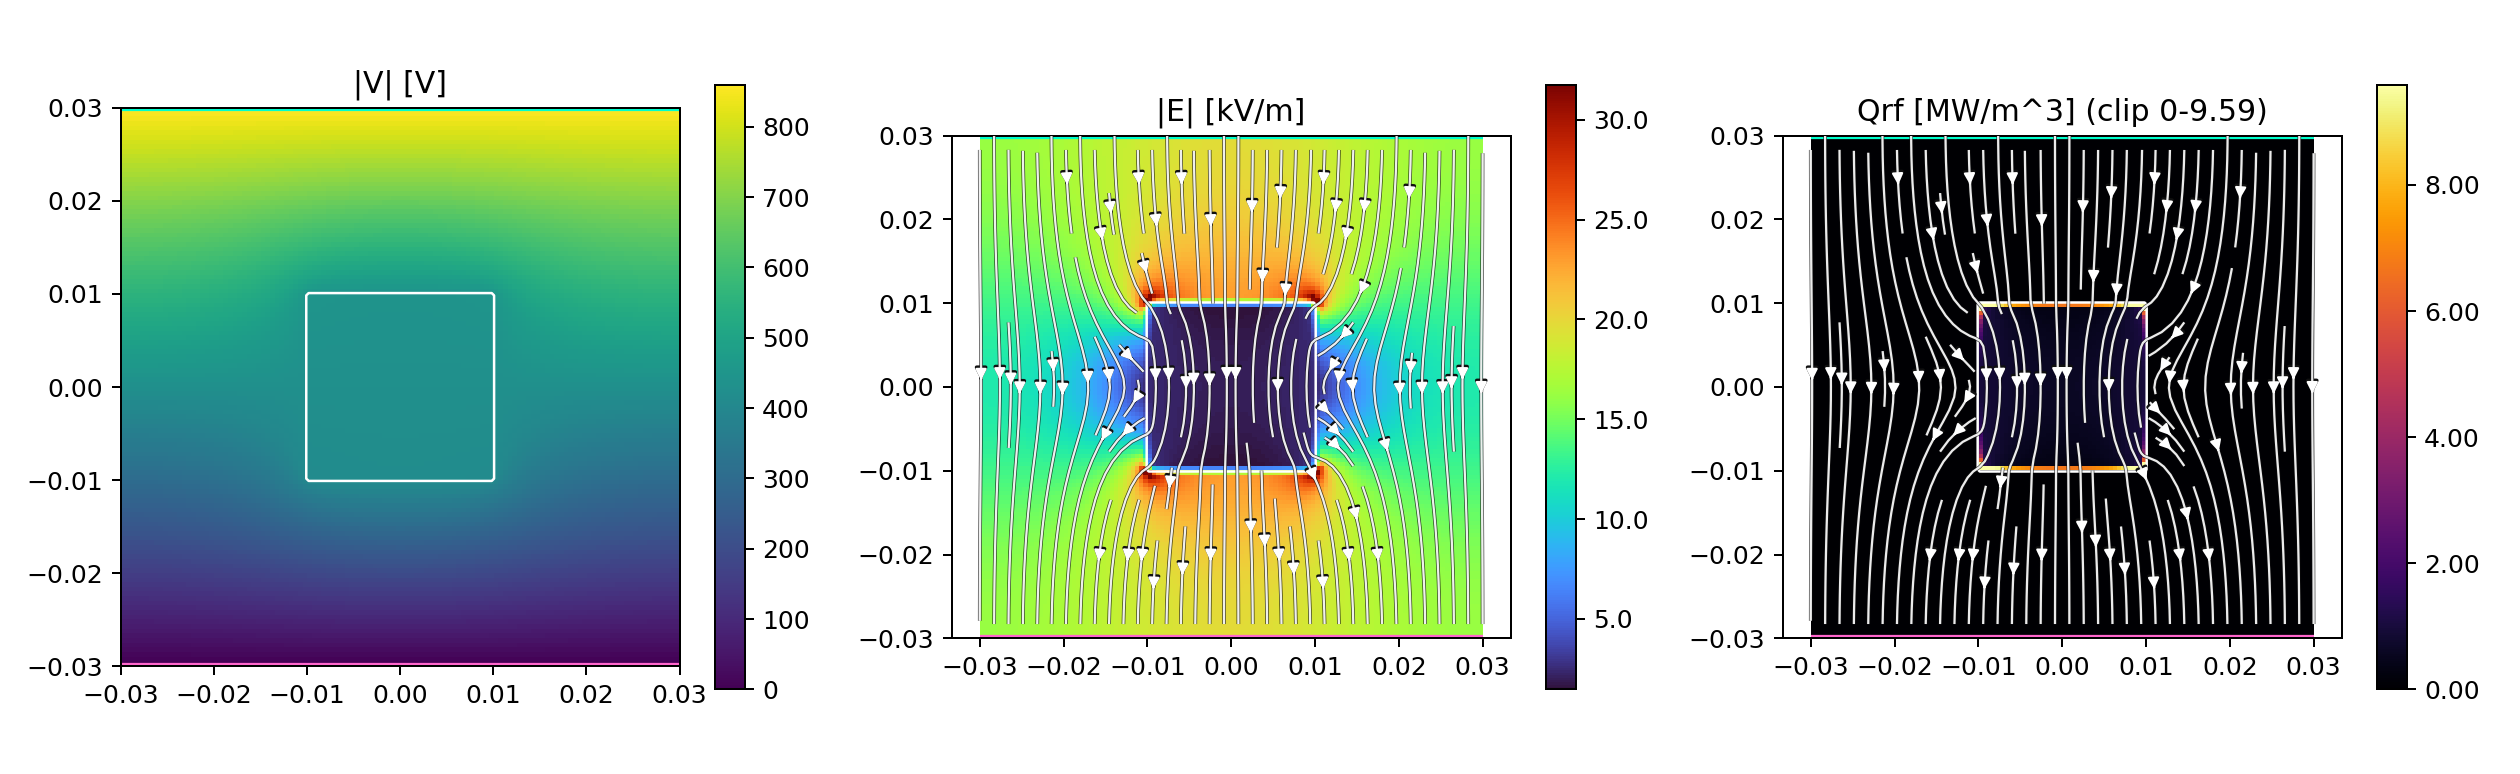
\includegraphics[width=0.86\linewidth]{fig_electric_fields.png}
\end{frame}

\begin{frame}{Canonical Thermal + Density Response (6 min)}
  \centering
  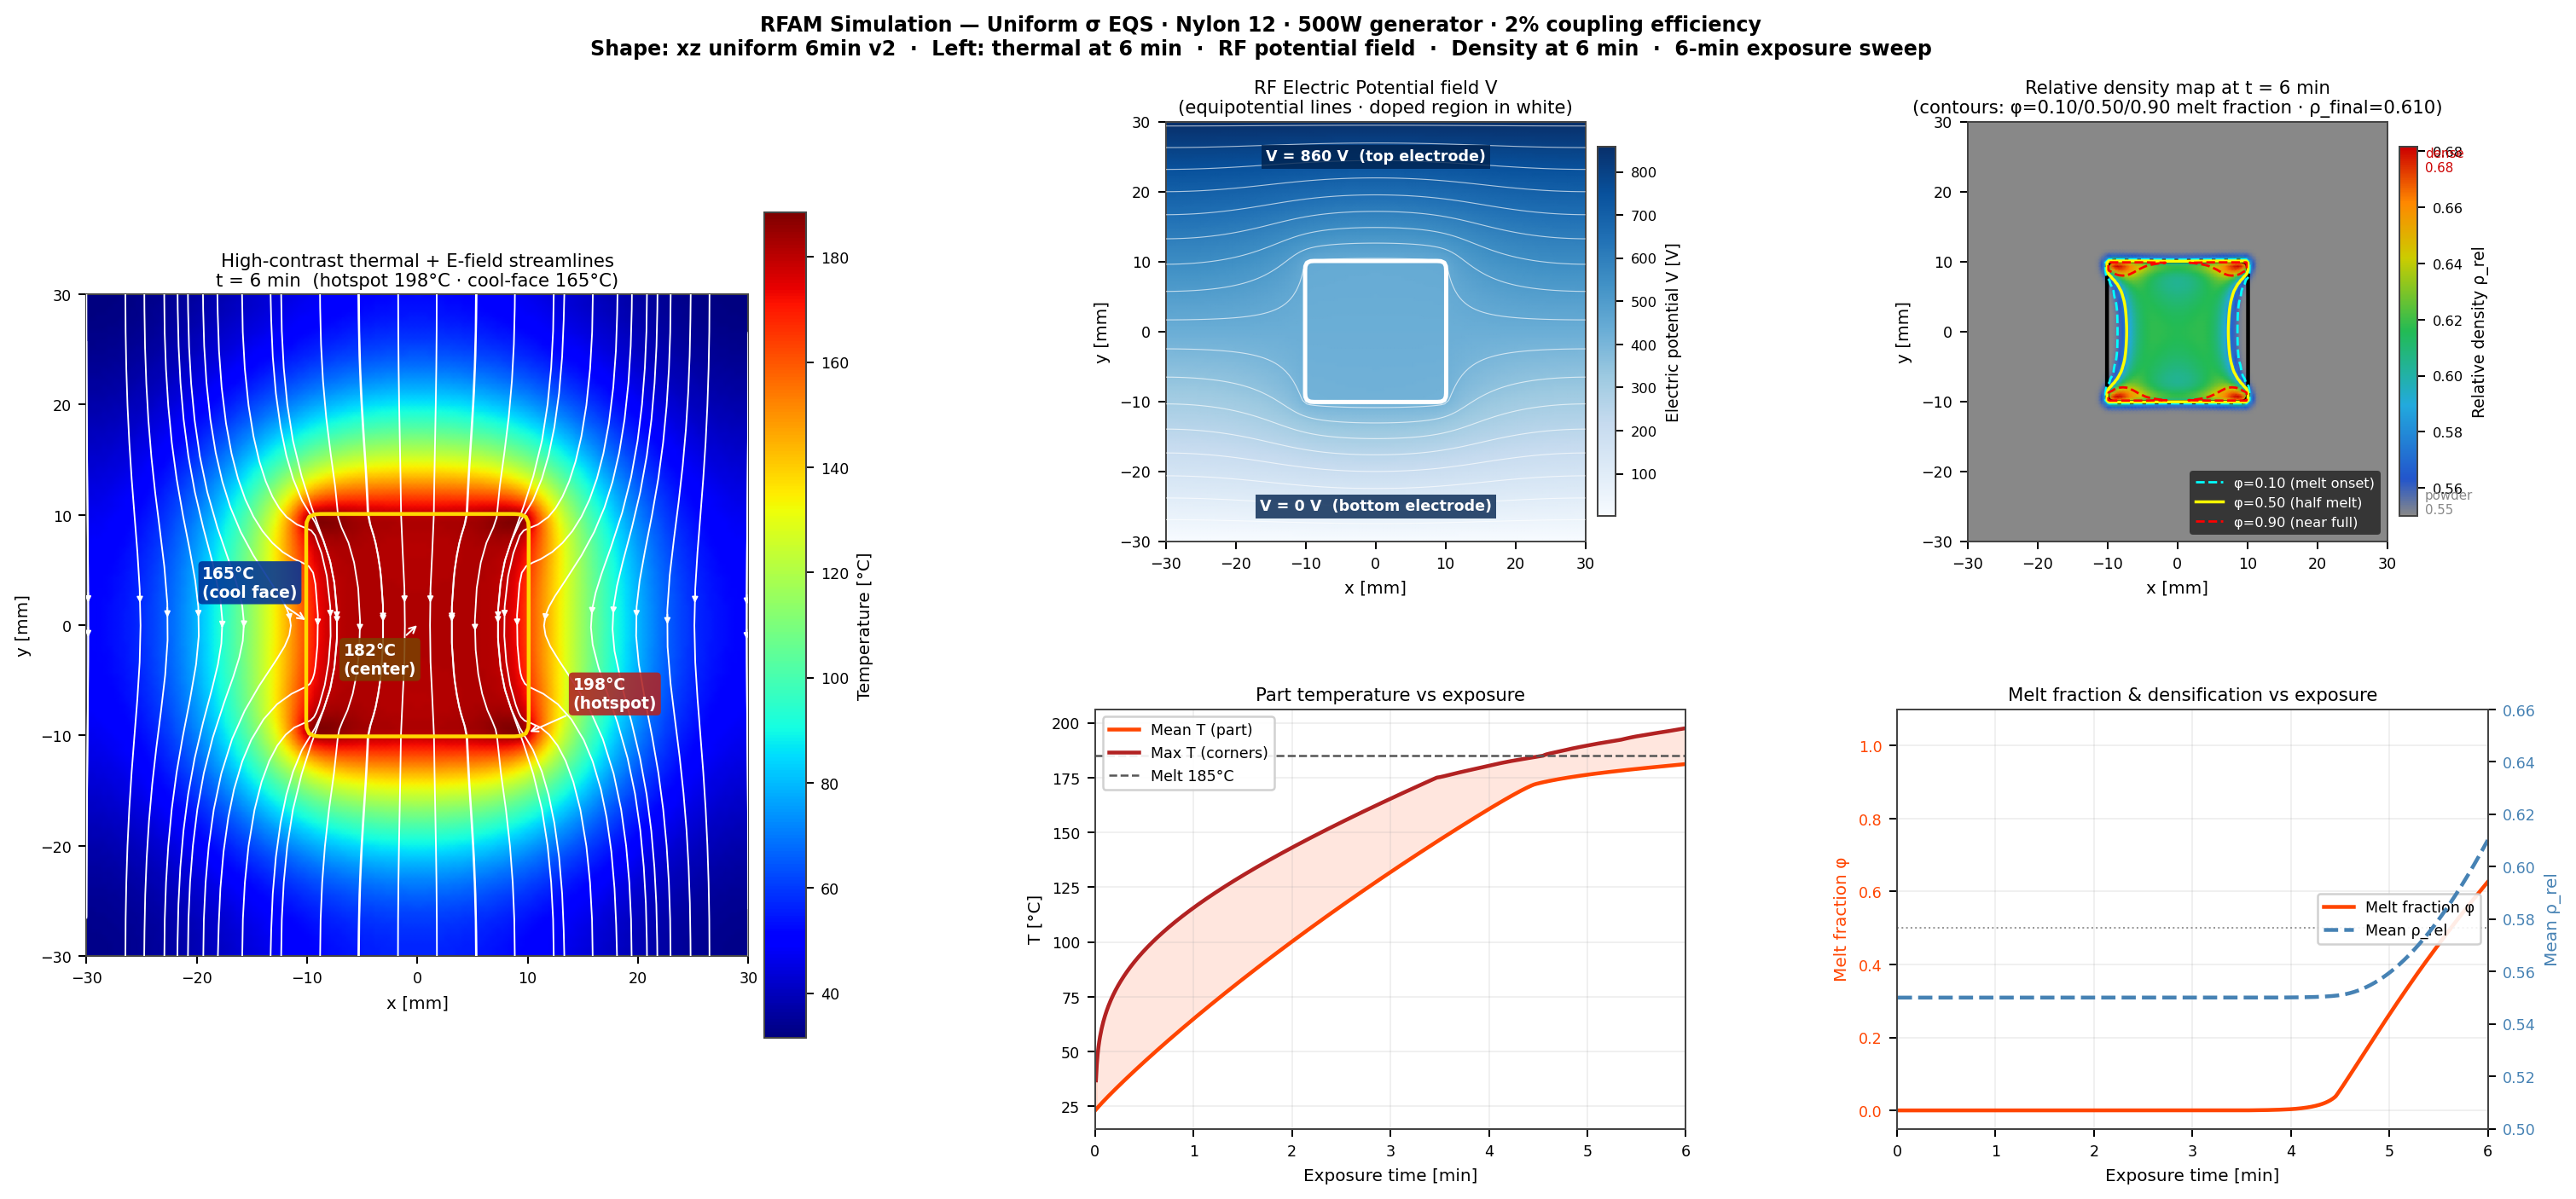
\includegraphics[width=\linewidth]{fig_canonical_v5.png}
\end{frame}

\begin{frame}{Forward Model (EQS + Thermal + Densification)}
  \small
  \begin{align*}
    \nabla \cdot (\sigma \nabla V) &= 0,\\
    \rho c_p^{\mathrm{eff}} \frac{\partial T}{\partial t} &= \nabla \cdot (k \nabla T) + \Qrf - h_c(T-T_\infty)\delta_{\mathrm{top}},\\
    \frac{d\rhorel}{dt} &= \left.\frac{d\rhorel}{dt}\right|_{\mathrm{ss}} + \left.\frac{d\rhorel}{dt}\right|_{\mathrm{liq}}.
  \end{align*}
  \normalsize
  \begin{itemize}
    \item Domain: $60 \times \SI{60}{\milli\meter}$, part: $20 \times \SI{20}{\milli\meter}$
    \item Generator: \SI{500}{\watt}, calibrated coupling $\eta = 0.020$
    \item Exposure baseline: \SI{360}{\second} (\SI{6}{\minute})
  \end{itemize}
\end{frame}

\begin{frame}{EPE-Based Prewarp Algorithm}
  \small
  \begin{align*}
    \EPE[i] &= (T[i]-\hat{B}[i])\cdot \hat{n}_i,\\
    P_{k+1}[i] &= P_k[i] + \alpha \EPE[i]\hat{n}_i.
  \end{align*}
  \normalsize
  \begin{itemize}
    \item Iterative loop: simulate $\rightarrow$ predict shrinkage $\rightarrow$ update polygon
    \item Effective shrinkage scale $\Leff$ calibrated per shape
    \item Stops when RMS(EPE) reaches tolerance
  \end{itemize}
\end{frame}

\begin{frame}{\texorpdfstring{$\Leff$}{Leff} Calibration}
  \centering
  \begin{columns}
    \column{0.5\linewidth}
    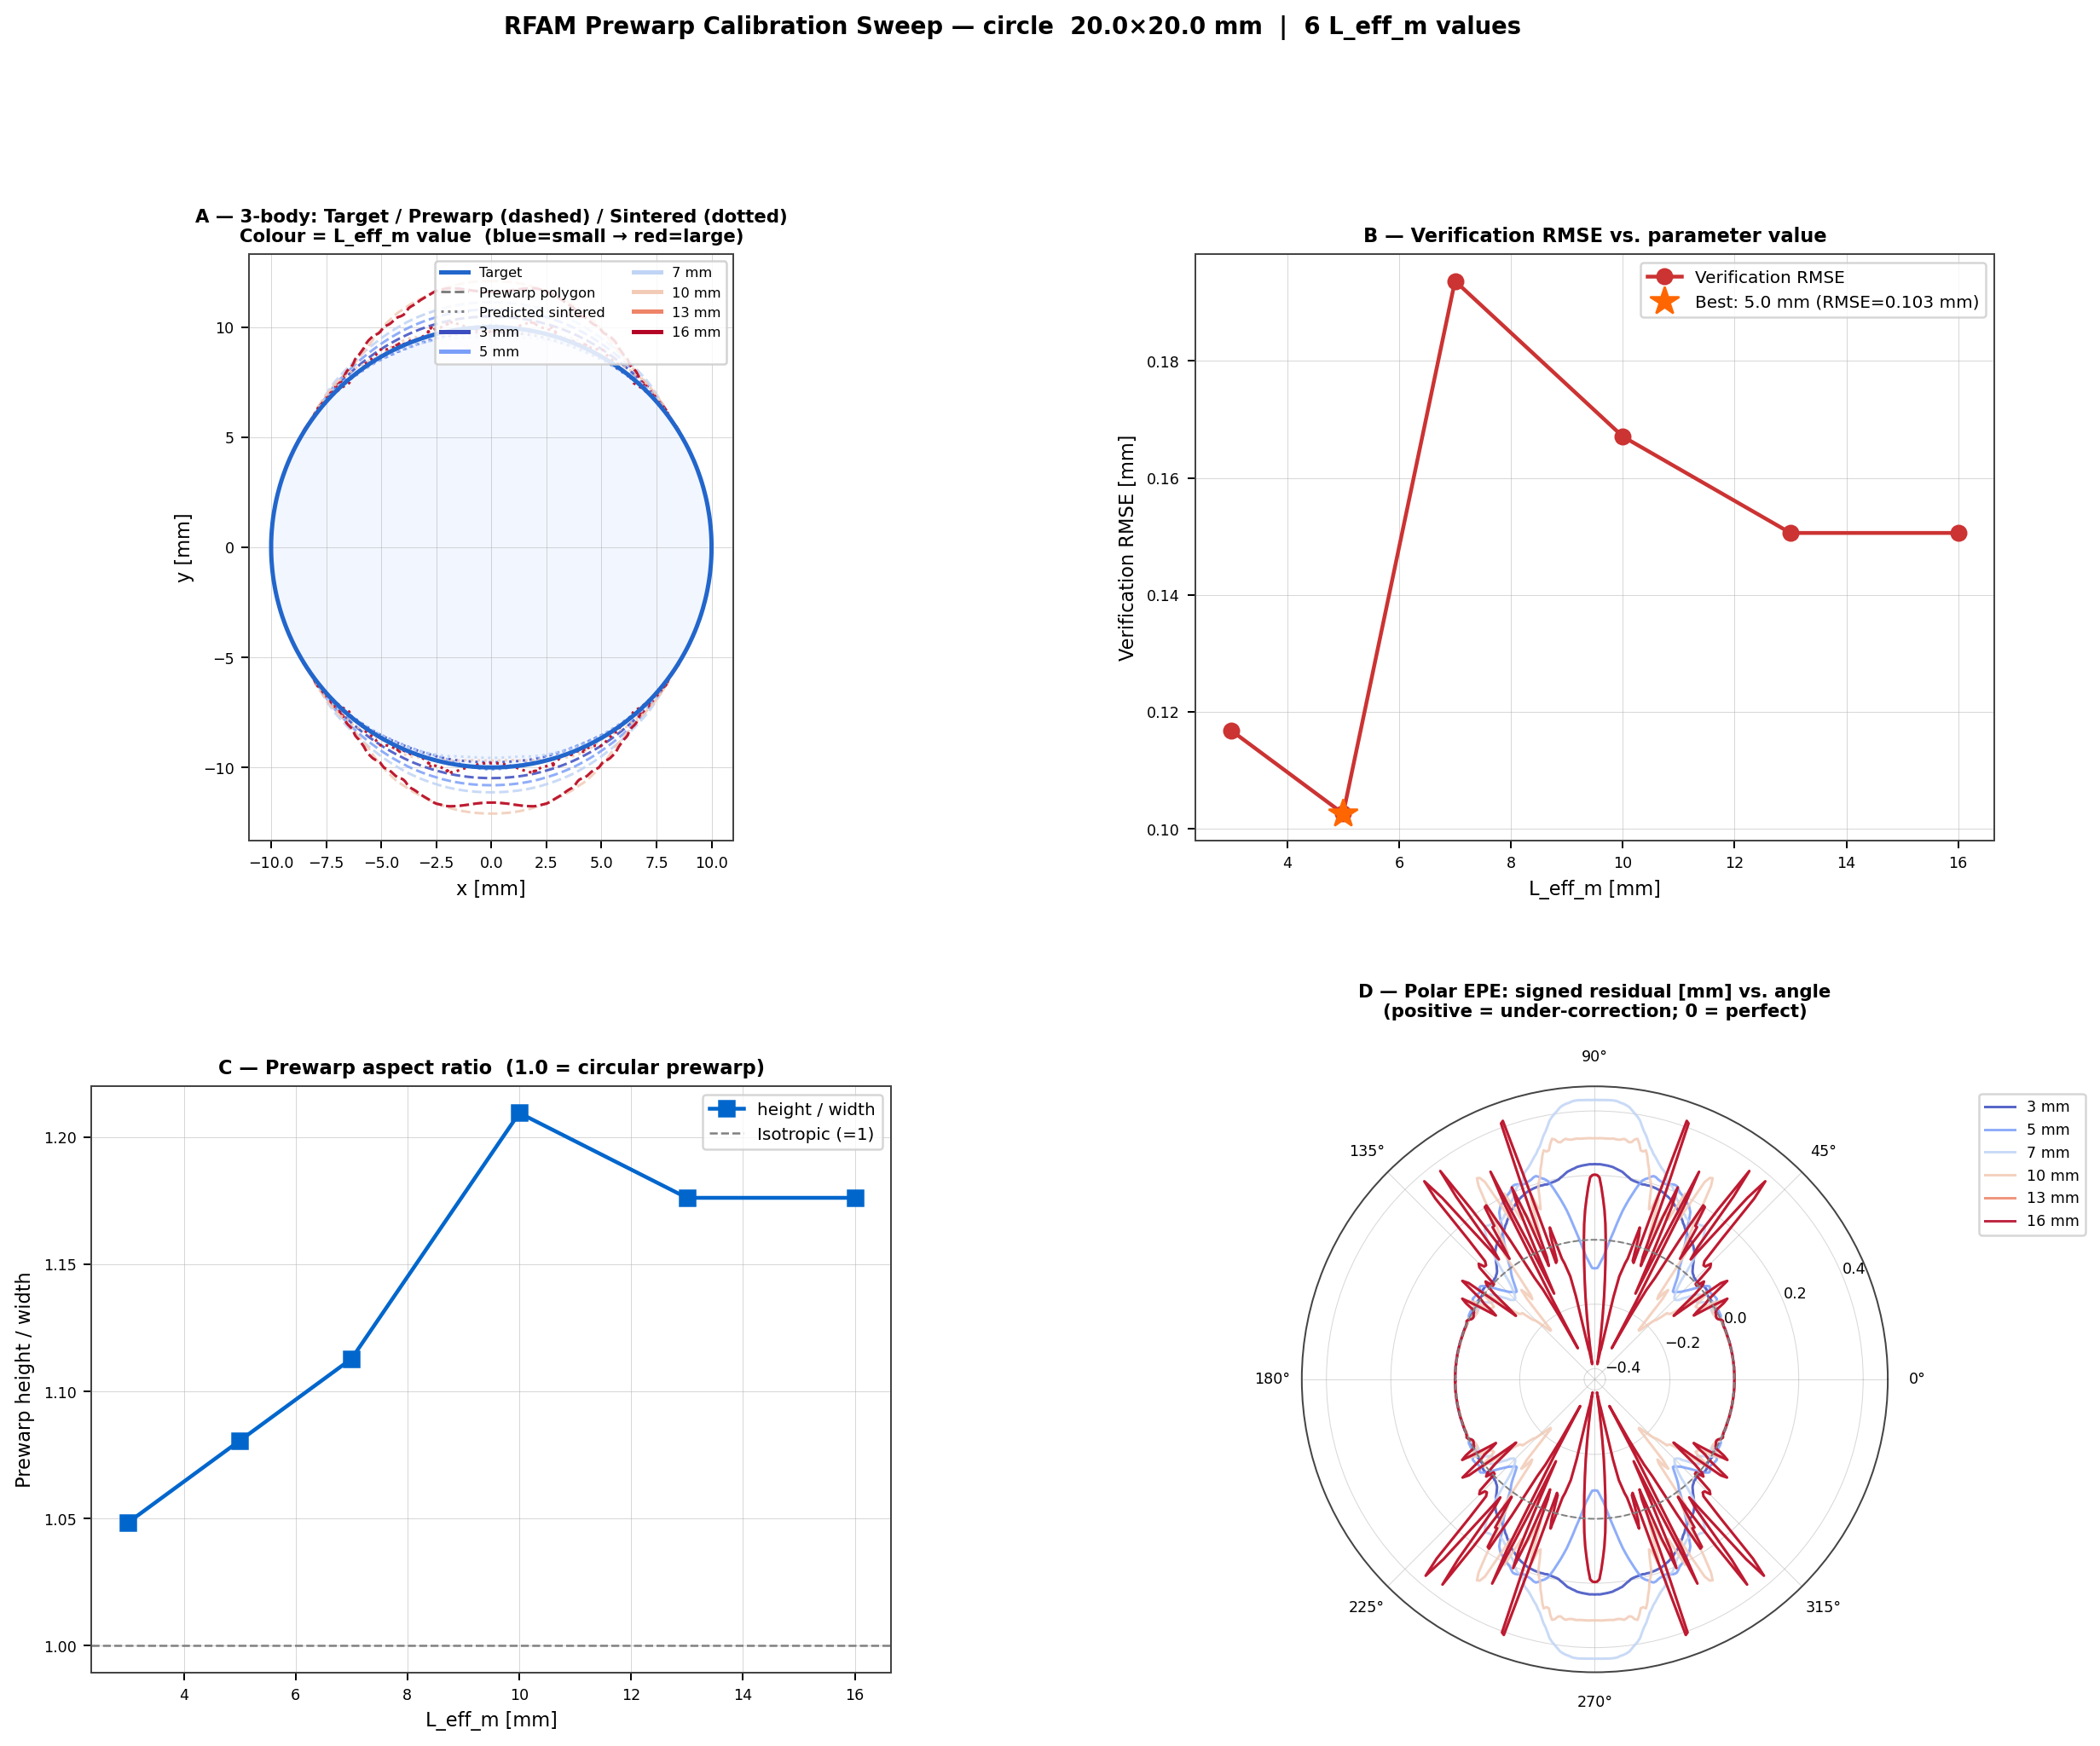
\includegraphics[width=\linewidth]{fig_calib_circle.png}
    \column{0.5\linewidth}
    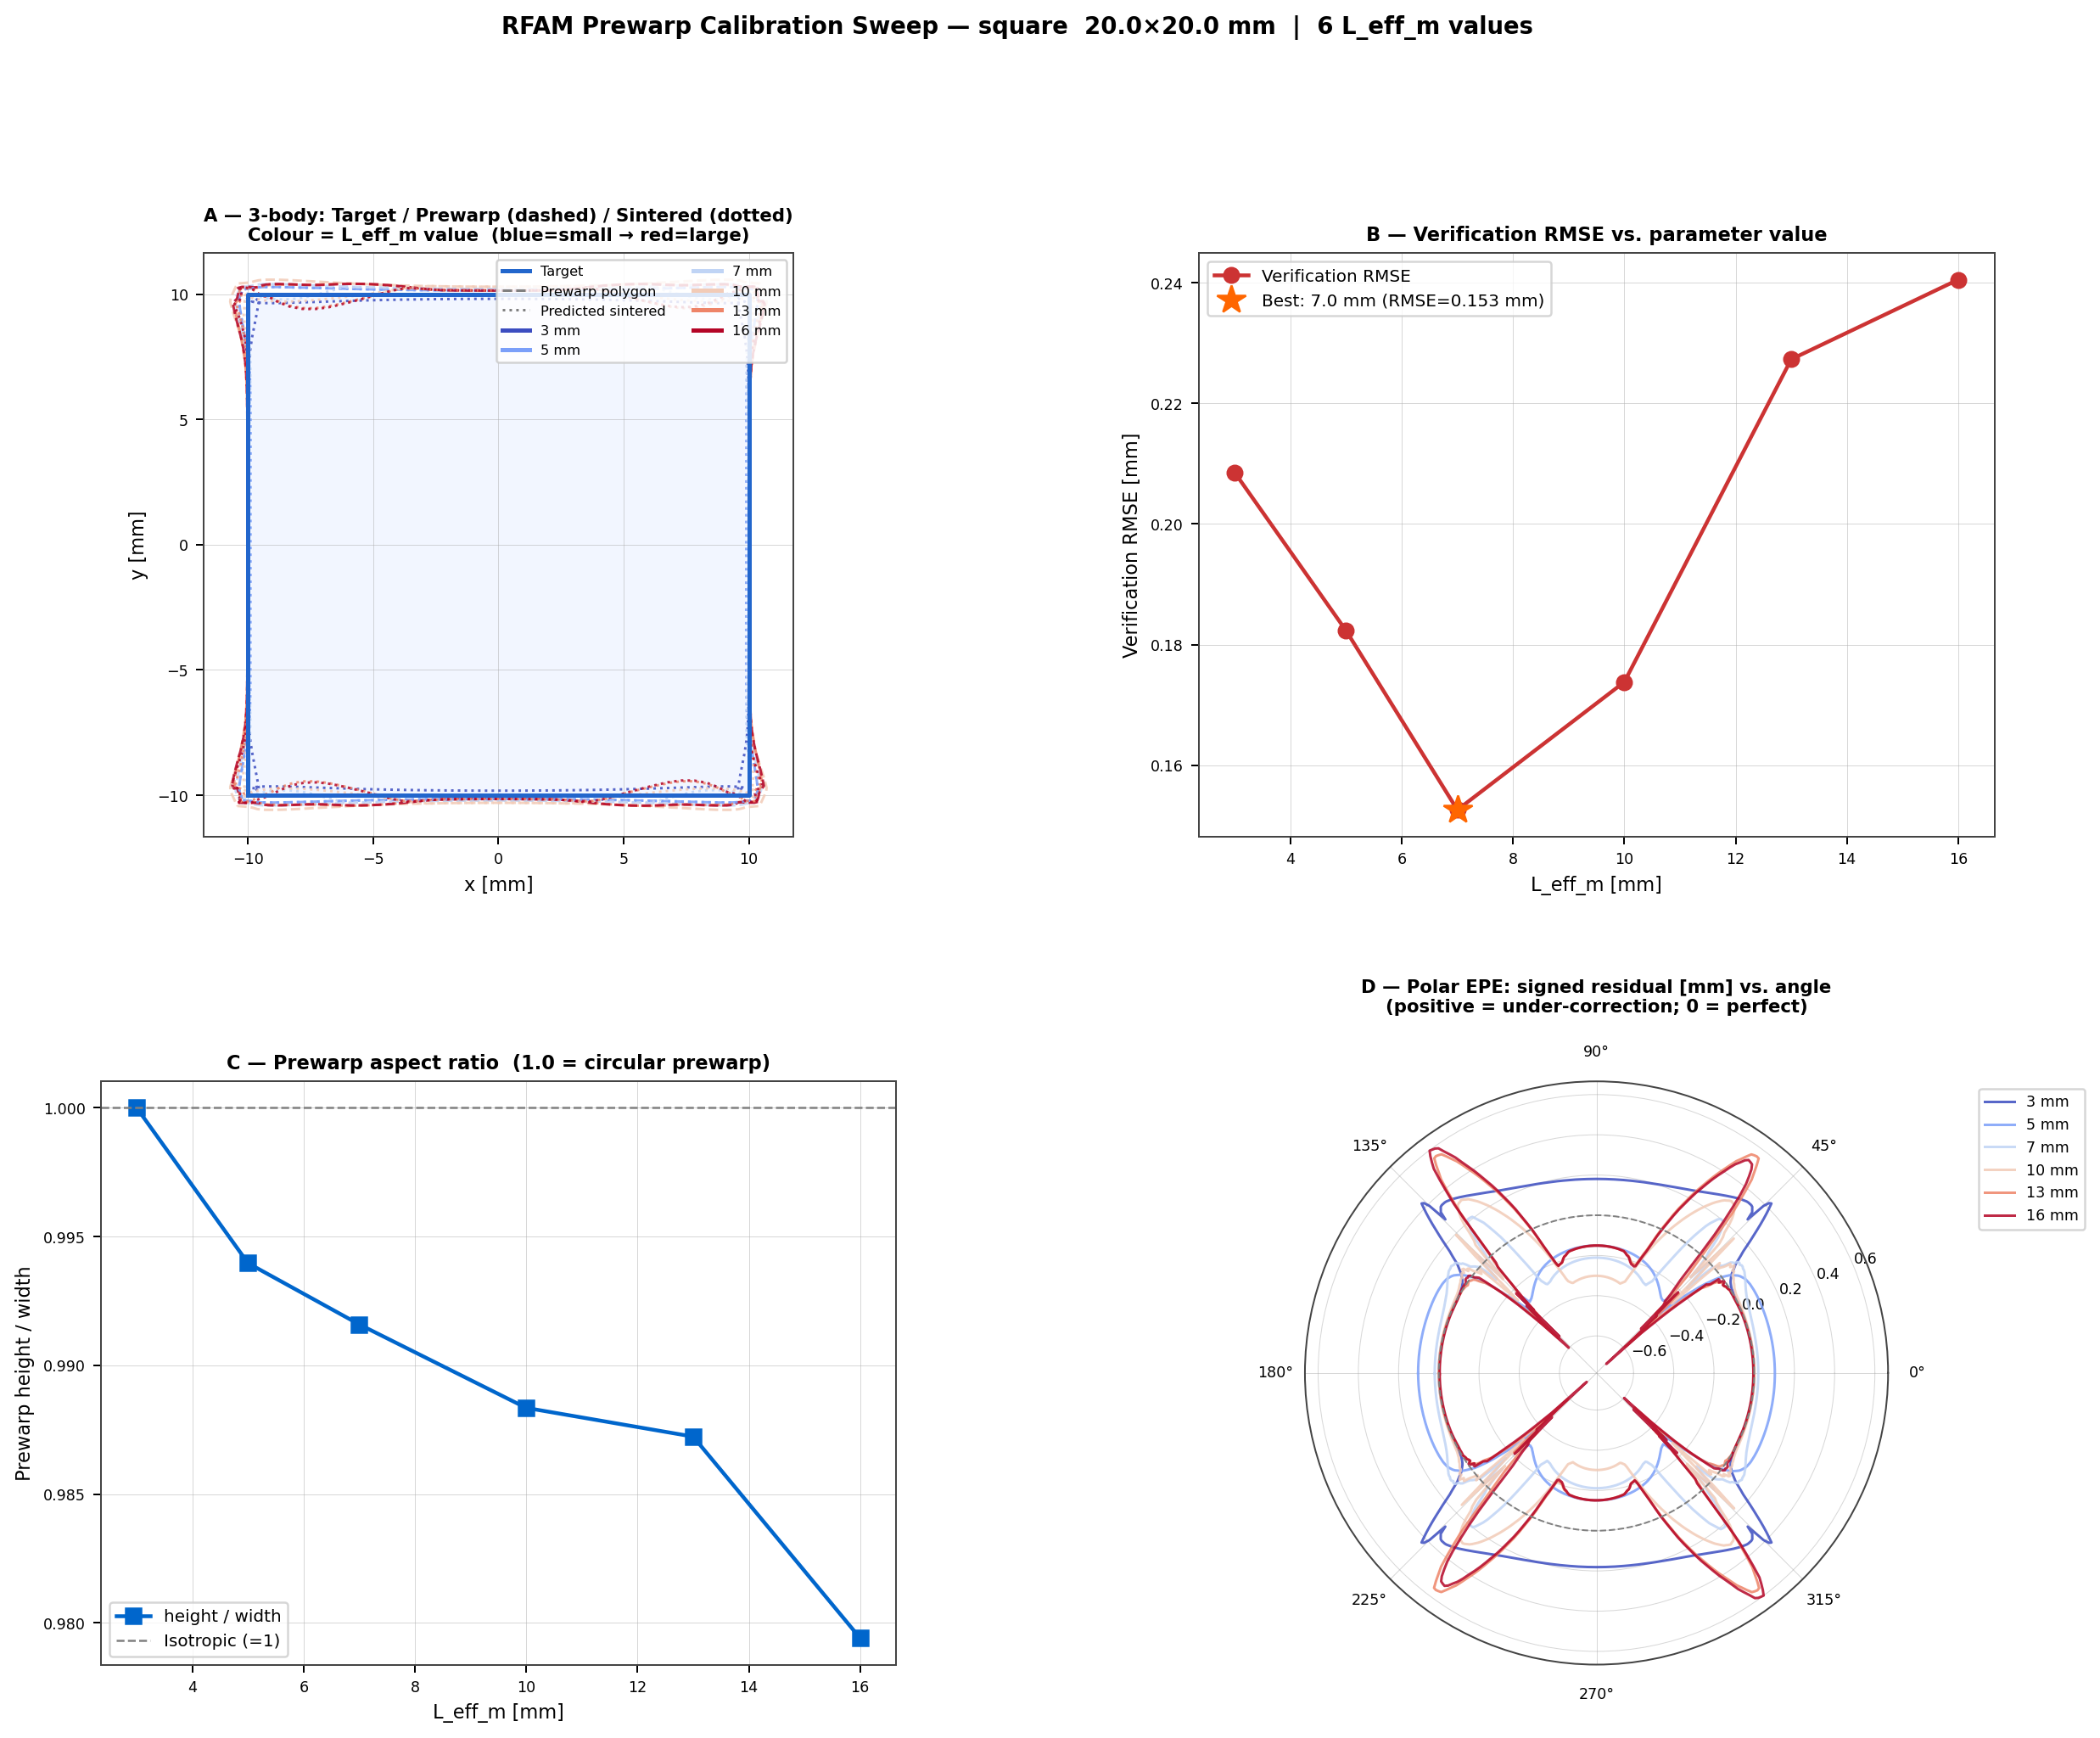
\includegraphics[width=\linewidth]{fig_calib_square.png}
  \end{columns}
  \vspace{0.5em}
  \small Optimal values: circle \SI{5}{\milli\meter}, square \SI{7}{\milli\meter}
\end{frame}

\begin{frame}{Square Prewarp Validation}
  \centering
  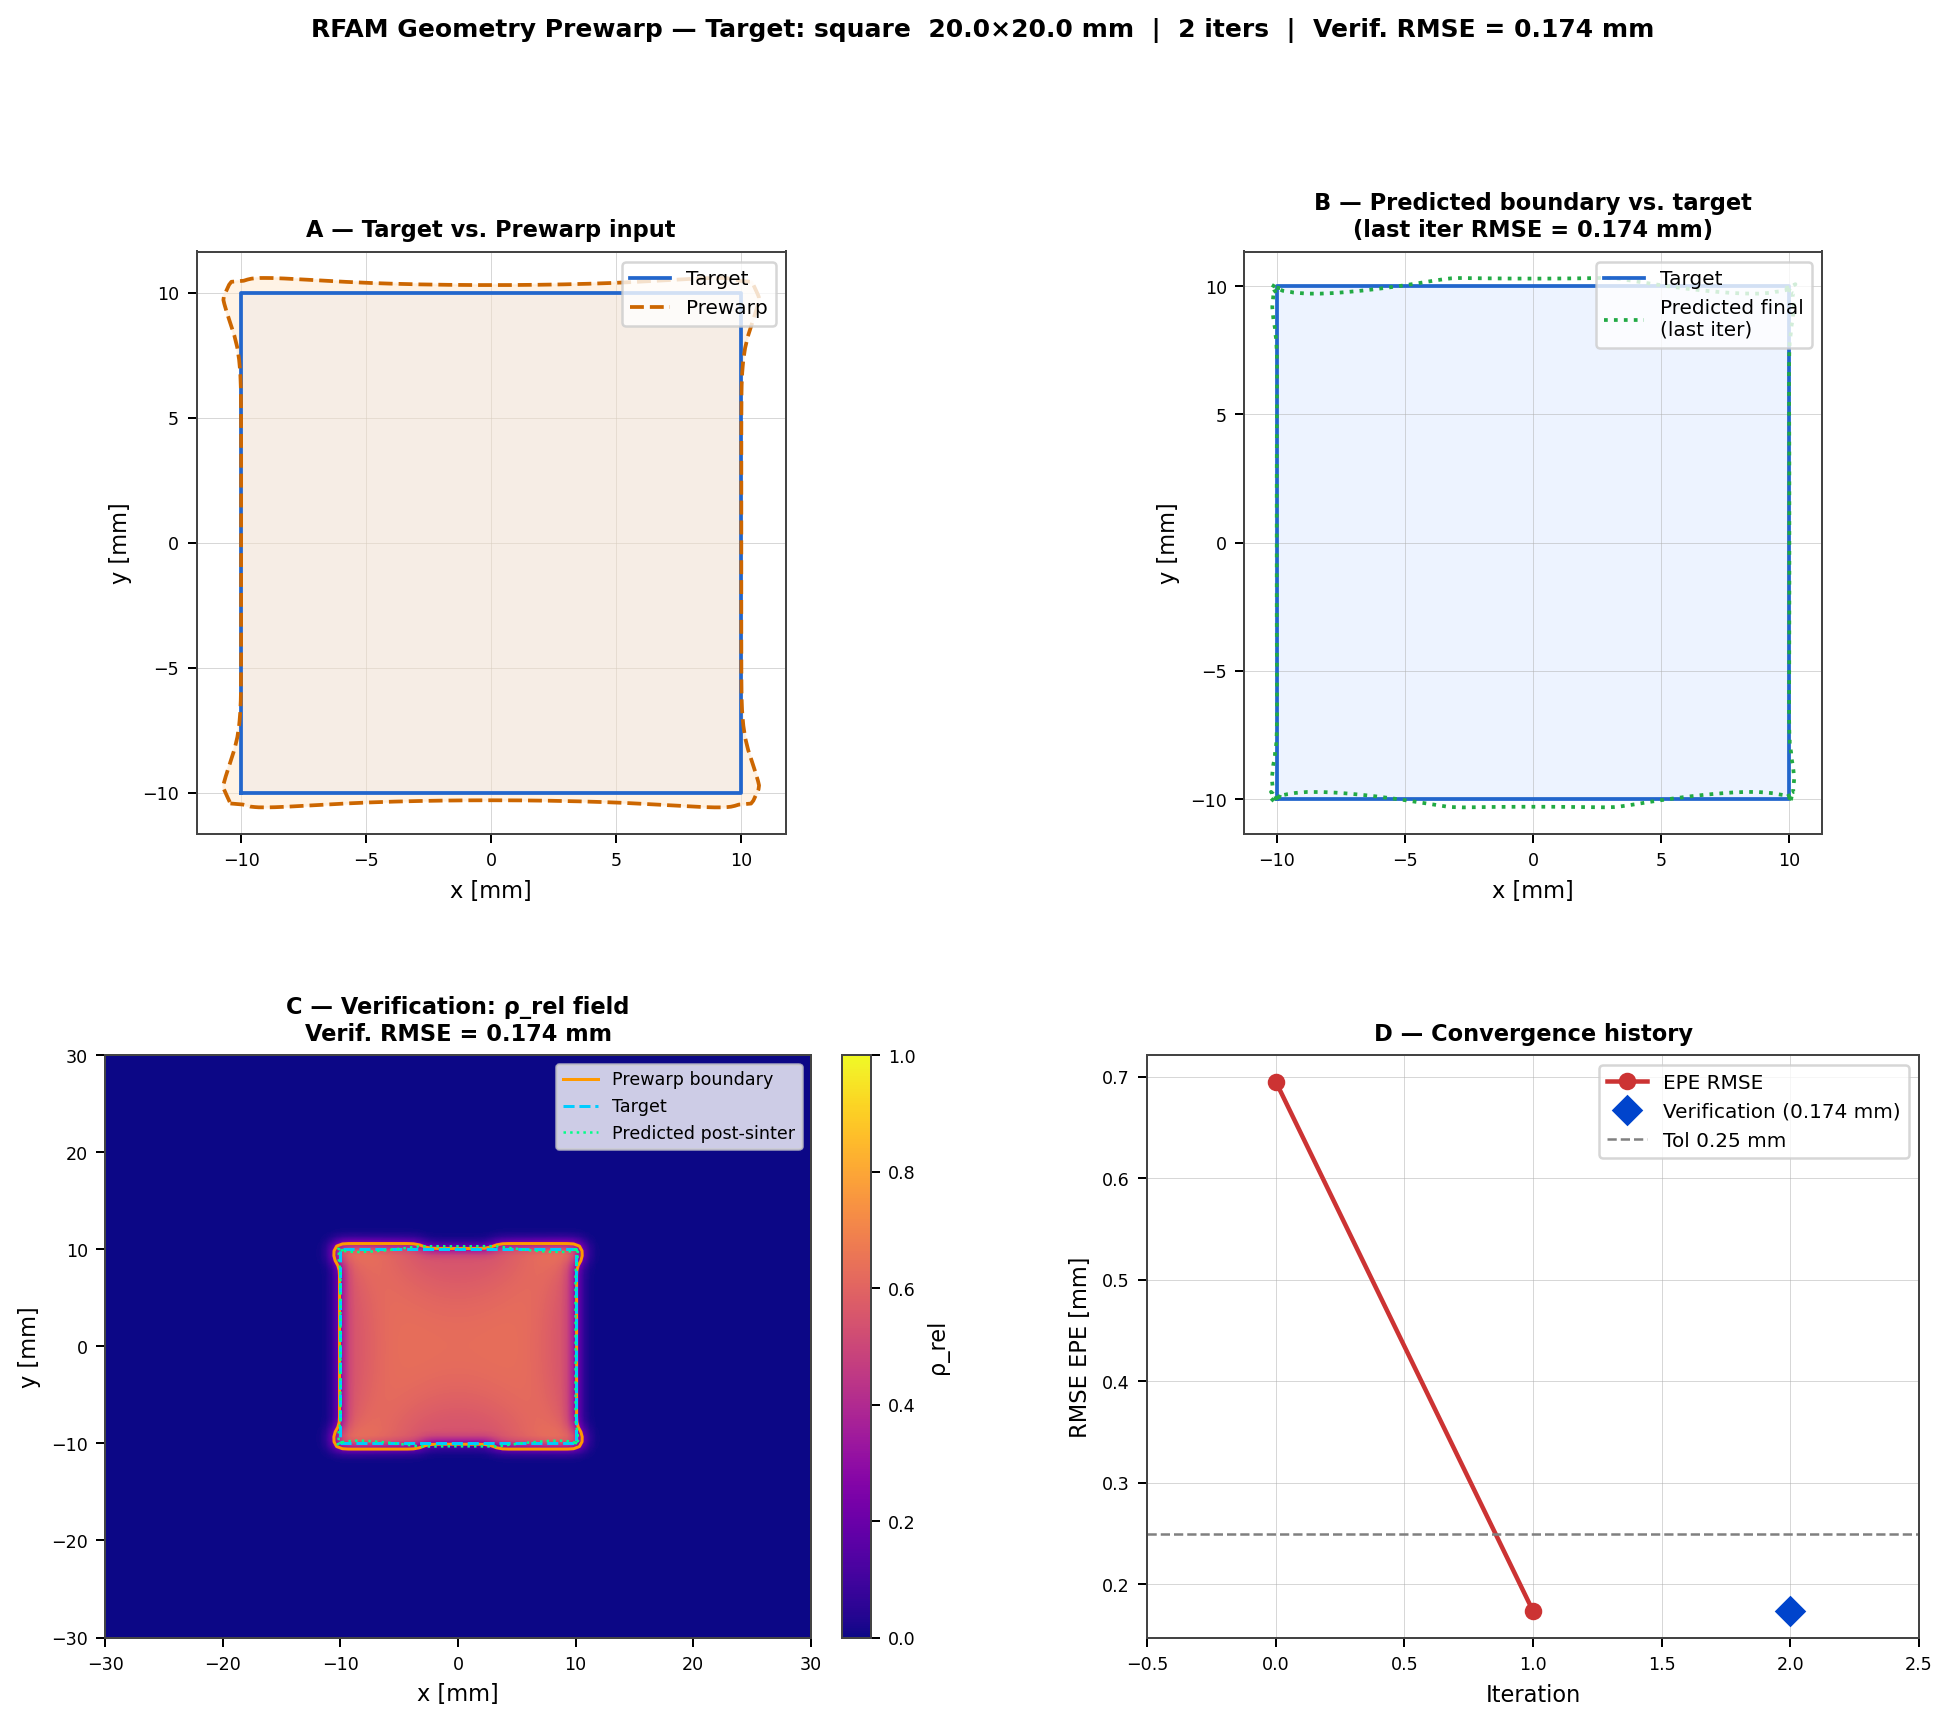
\includegraphics[width=0.82\linewidth]{fig_prewarp_square.png}
  \vspace{0.4em}
  \begin{itemize}
    \item RMSE: \SI{0.37}{\milli\meter} $\rightarrow$ \SI{0.153}{\milli\meter} (59\% reduction)
    \item Side effect: boundary uniformity also improves
  \end{itemize}
\end{frame}

\begin{frame}{Primitive Shape Library (17 Shapes)}
  \centering
  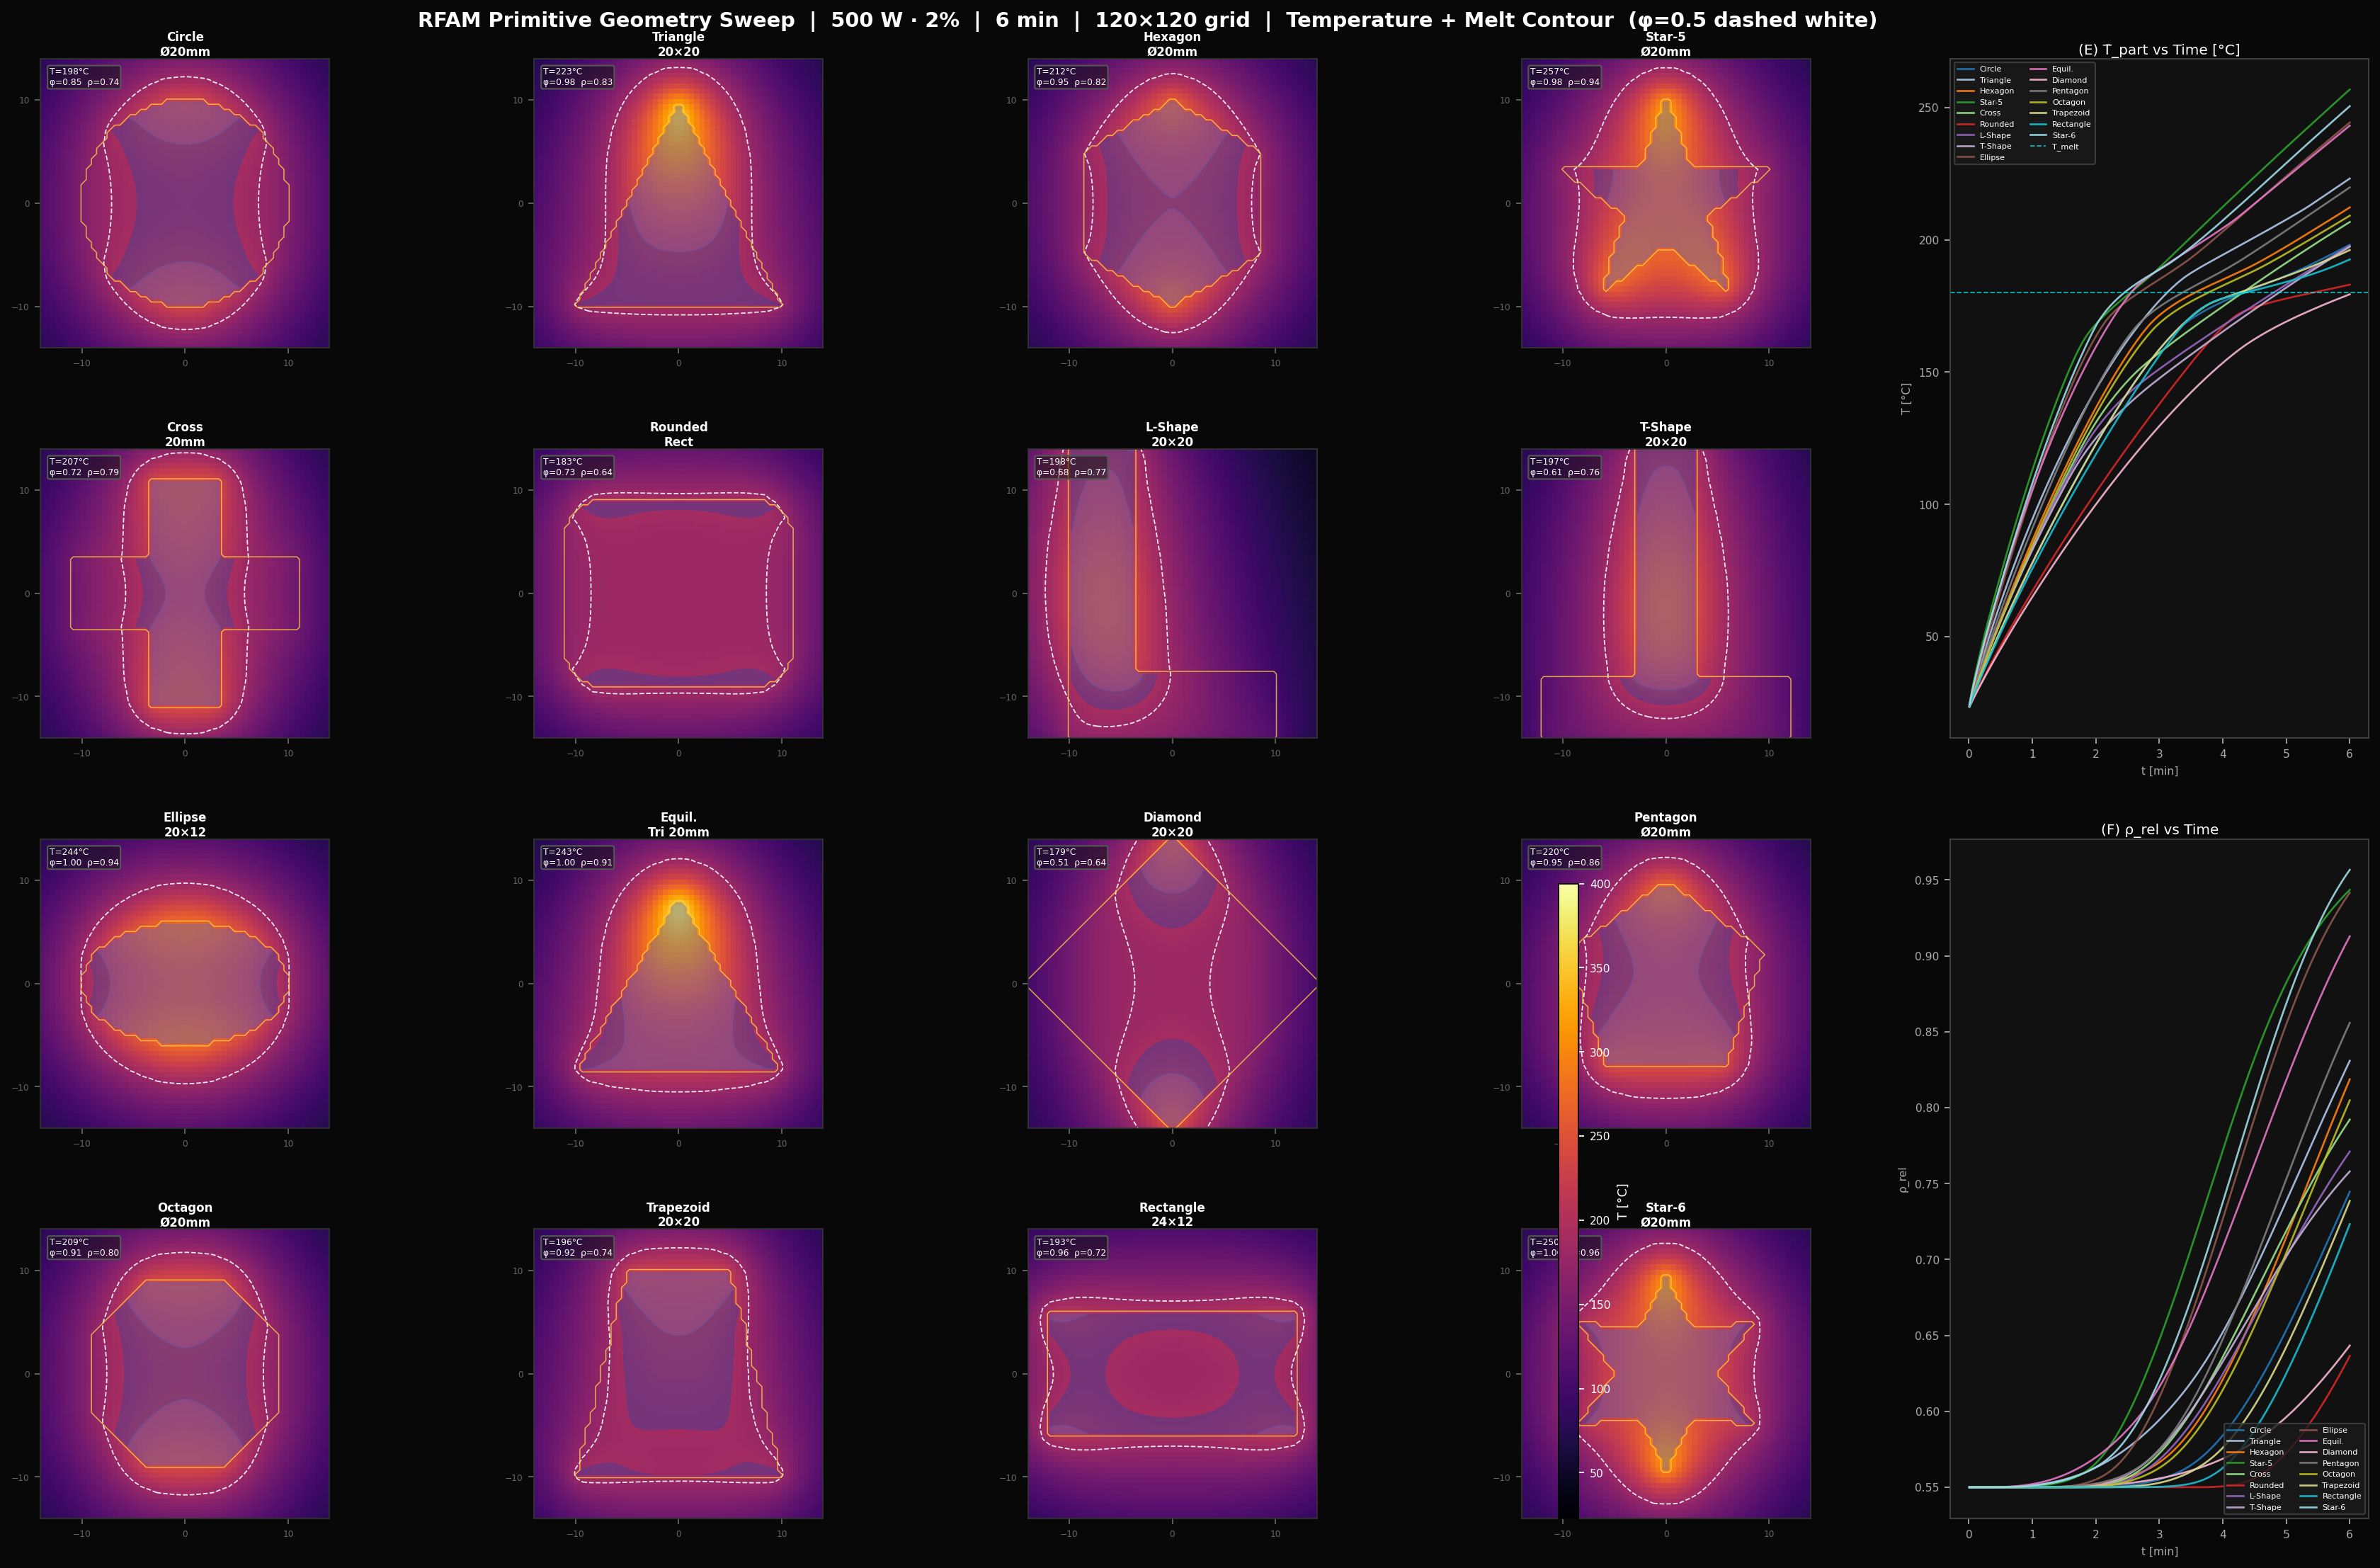
\includegraphics[width=\linewidth]{fig_primitive_sweep.png}
\end{frame}

\begin{frame}{Shape-Library Takeaways}
  \begin{itemize}
    \item Higher rotational symmetry generally reduces boundary non-uniformity.
    \item Concave/re-entrant features (L, T, Cross) increase shielding and worsen $\bndstd$.
    \item Diamond paradox: low mean heating but severe local tip hot-spots.
  \end{itemize}
\end{frame}

\begin{frame}{Spike Assist Features}
  \centering
  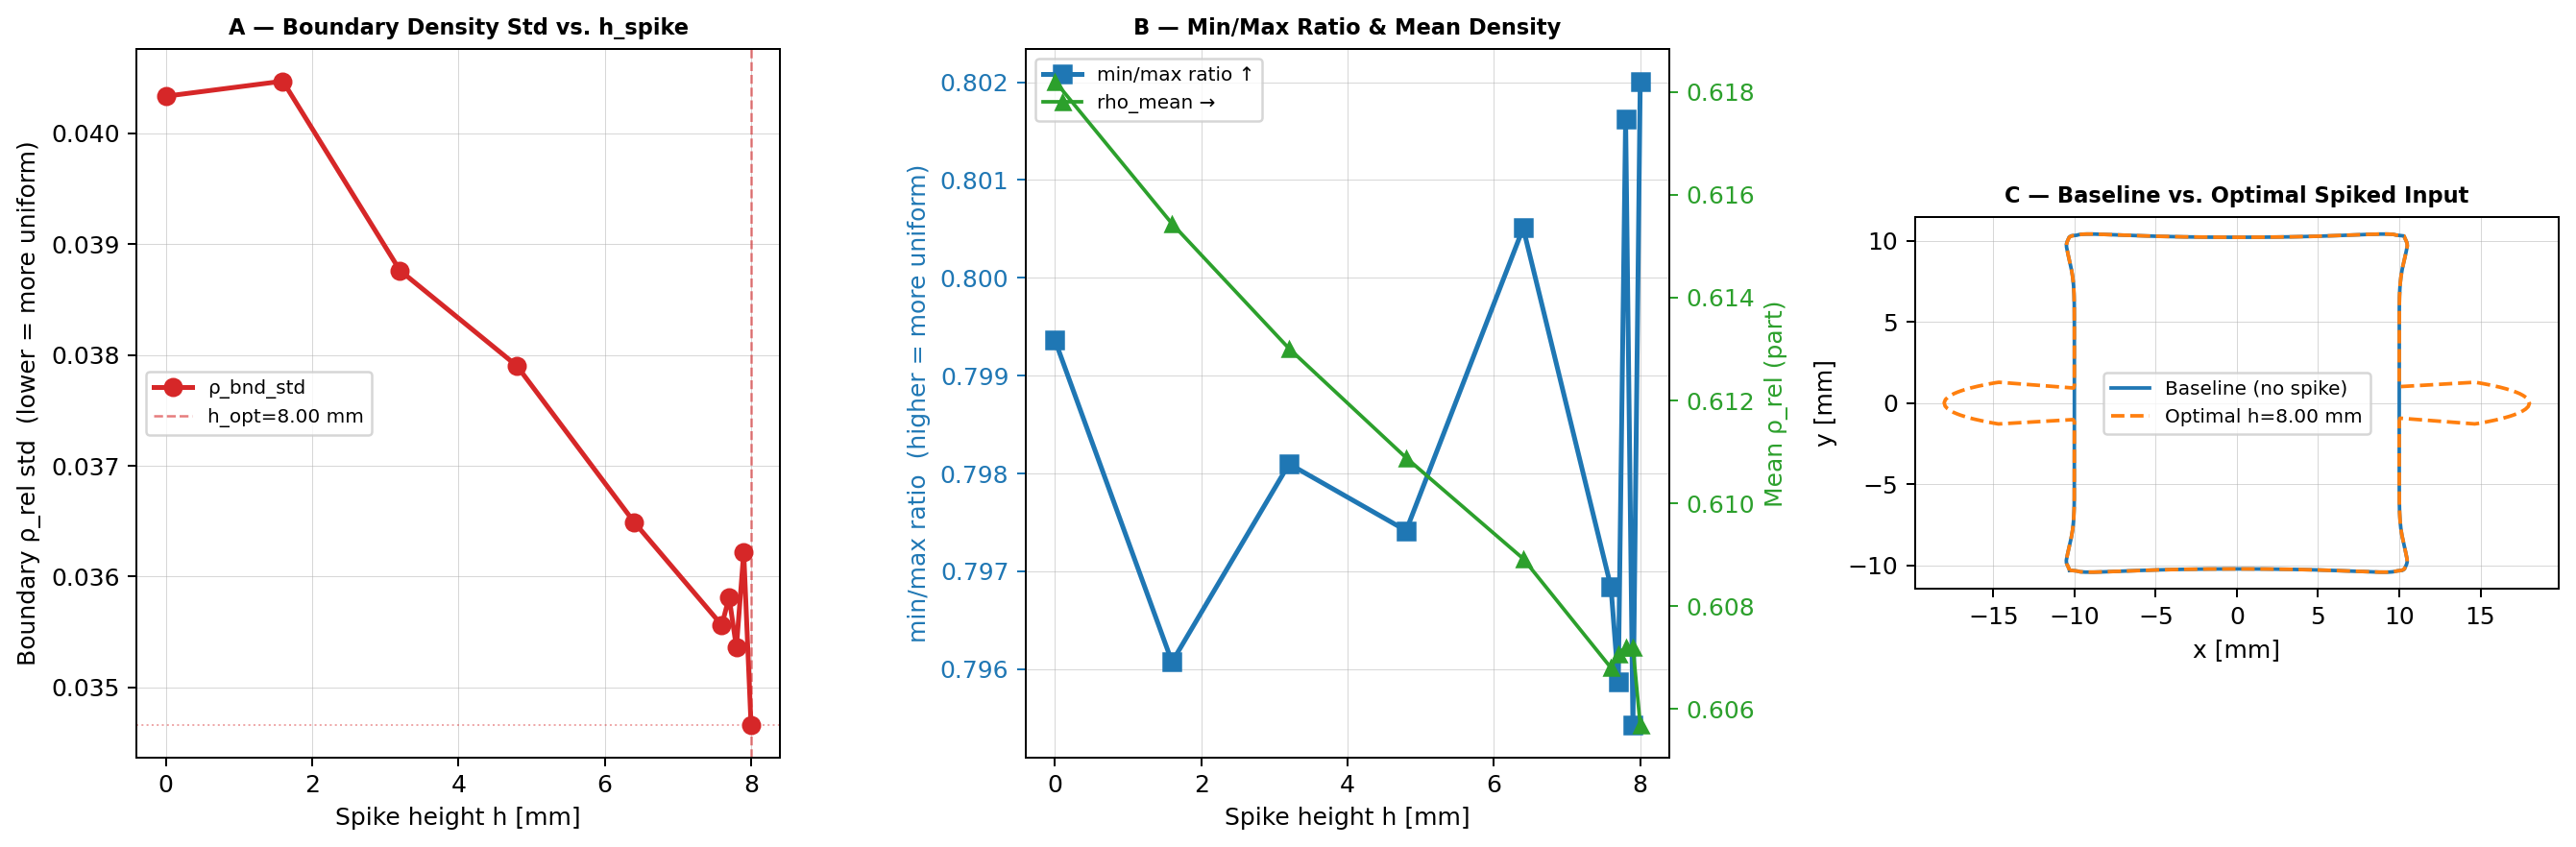
\includegraphics[width=0.82\linewidth]{fig_spike_coopt.png}
  \vspace{0.4em}
  \begin{itemize}
    \item Best case at $h=\SI{8}{\milli\meter}$ gives only 14.1\% $\bndstd$ improvement.
    \item Geometrically impractical and degrades target-shape RMSE.
  \end{itemize}
\end{frame}

\begin{frame}{Turntable Rotation Strategy}
  \begin{itemize}
    \item Discrete $90^\circ$ rotations average anisotropic exposure over time.
    \item 4-rotation schedule over 6 minutes:
    \[
      t_k=\frac{k}{N_r+1}t_{\mathrm{total}},
      \quad t_k=\{72,144,216,288\}\ \si{\second}
    \]
    \item Early/frequent rotation outperforms late single rotation.
  \end{itemize}
\end{frame}

\begin{frame}{Square: Uniformity Comparison}
  \centering
  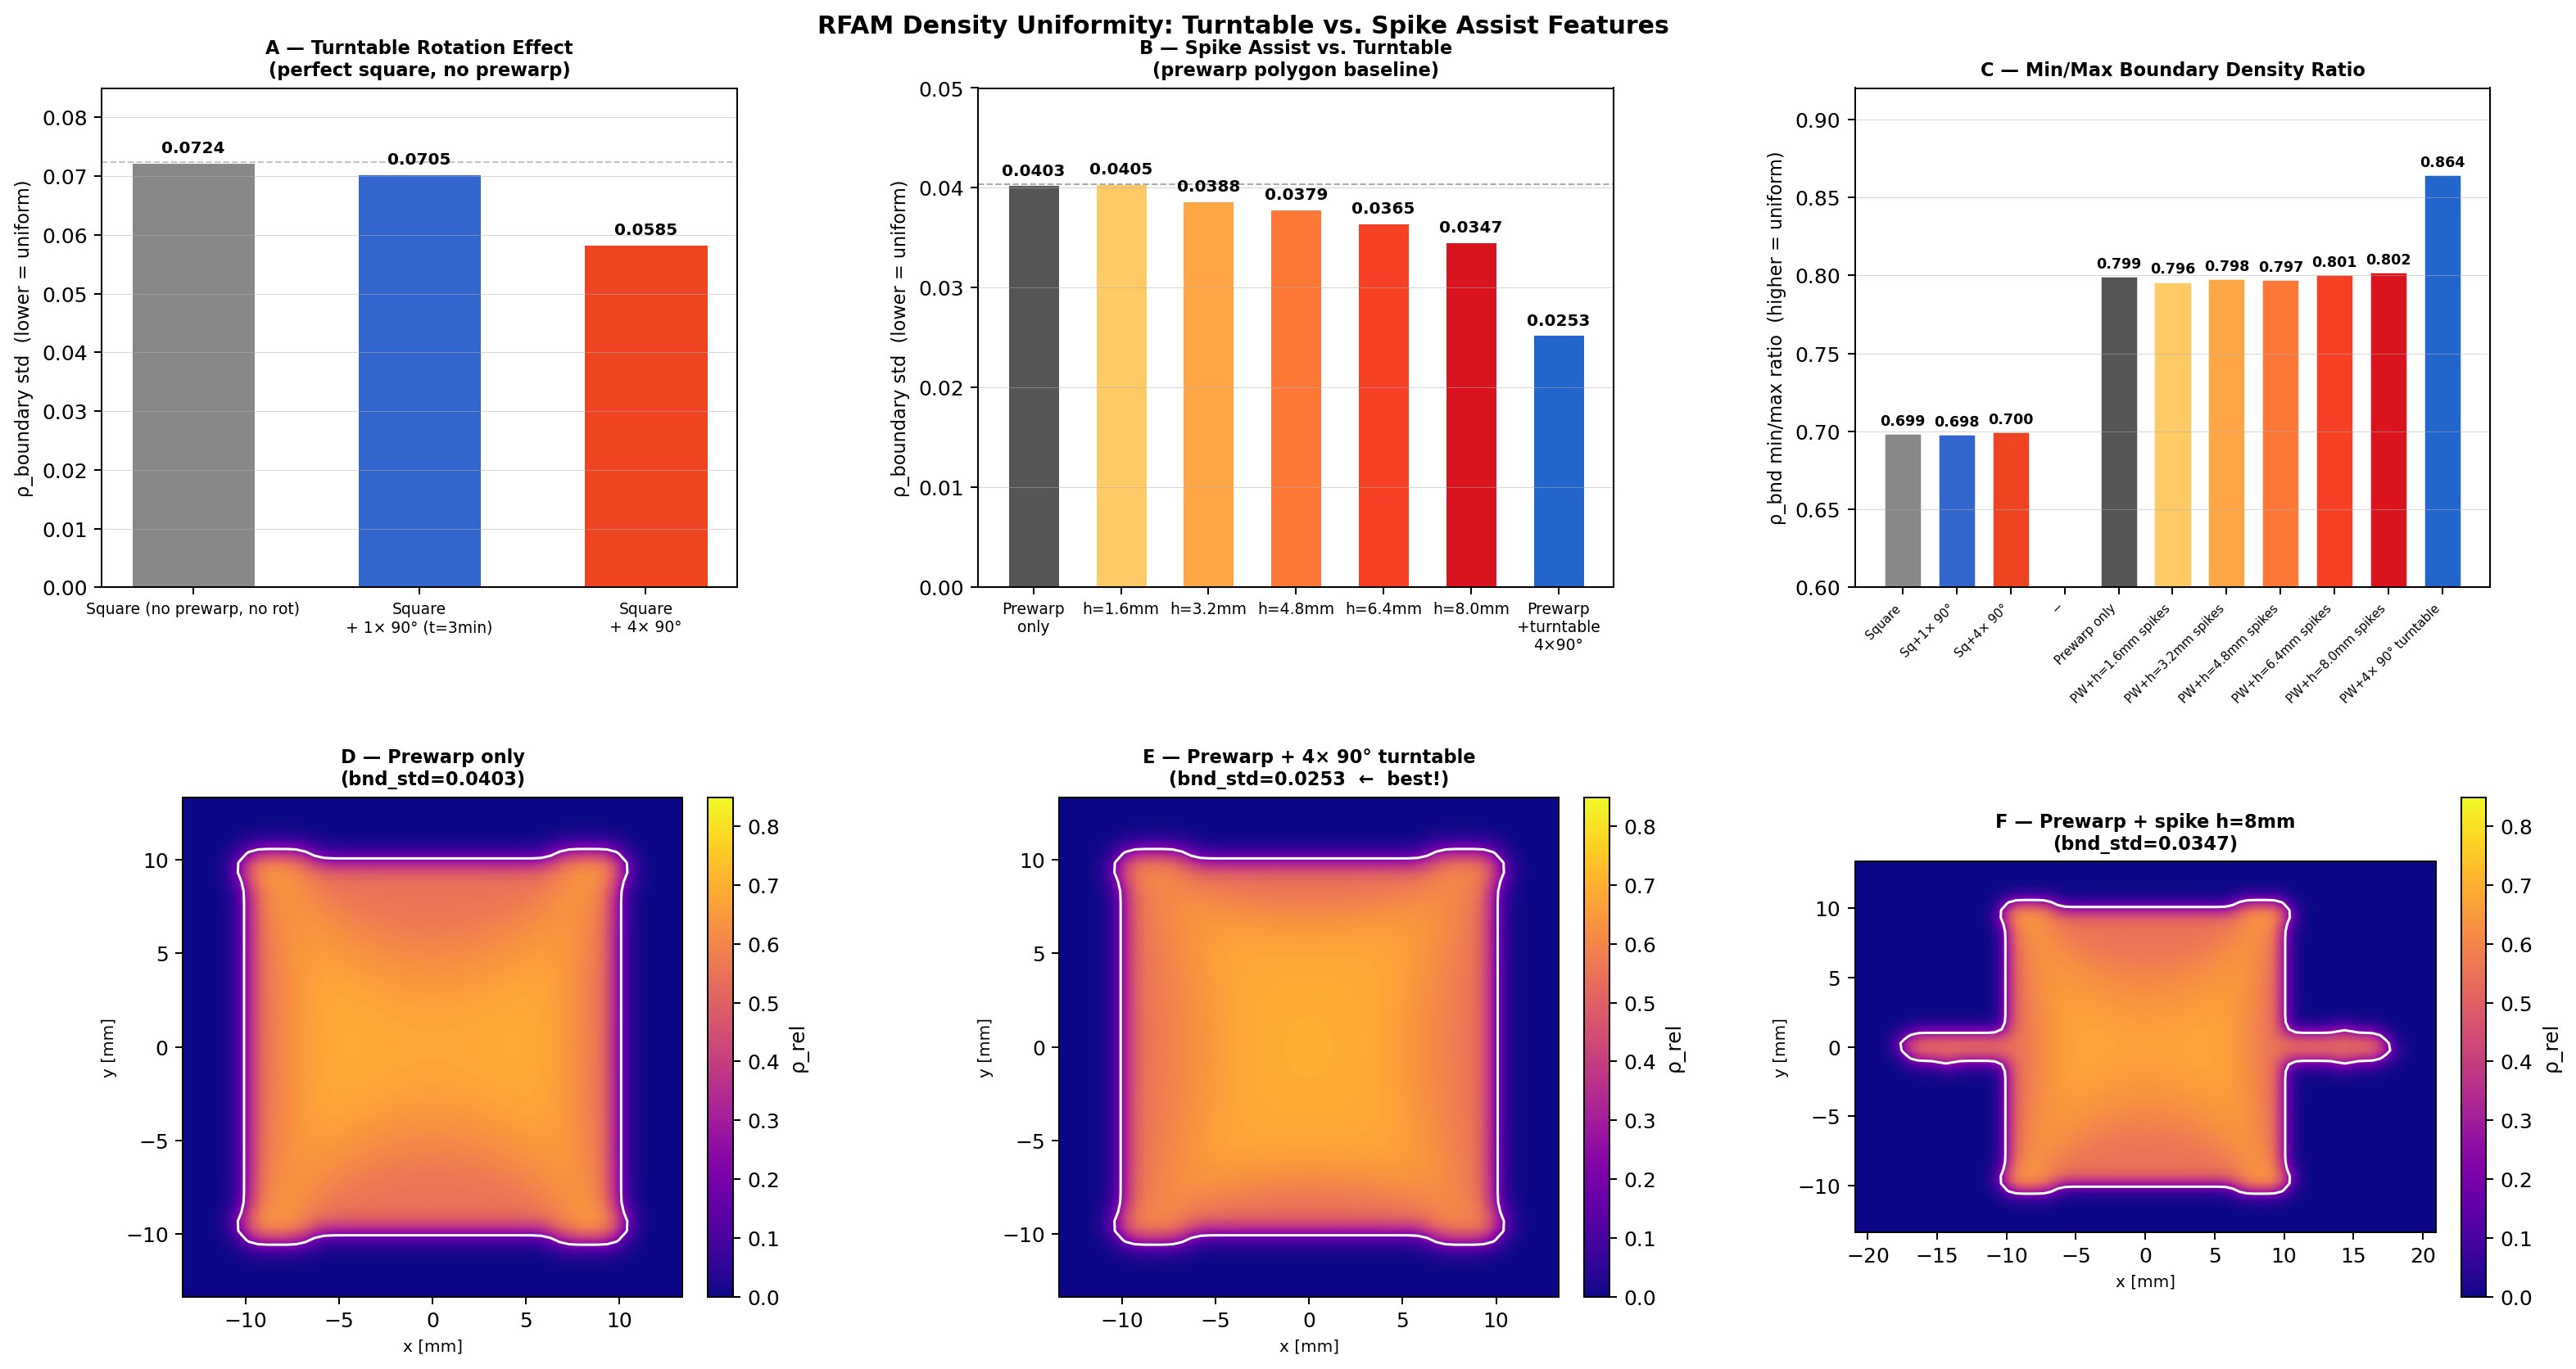
\includegraphics[width=\linewidth]{fig_uniformity_comparison.png}
\end{frame}

\begin{frame}{H-Shape Prewarp Result}
  \centering
  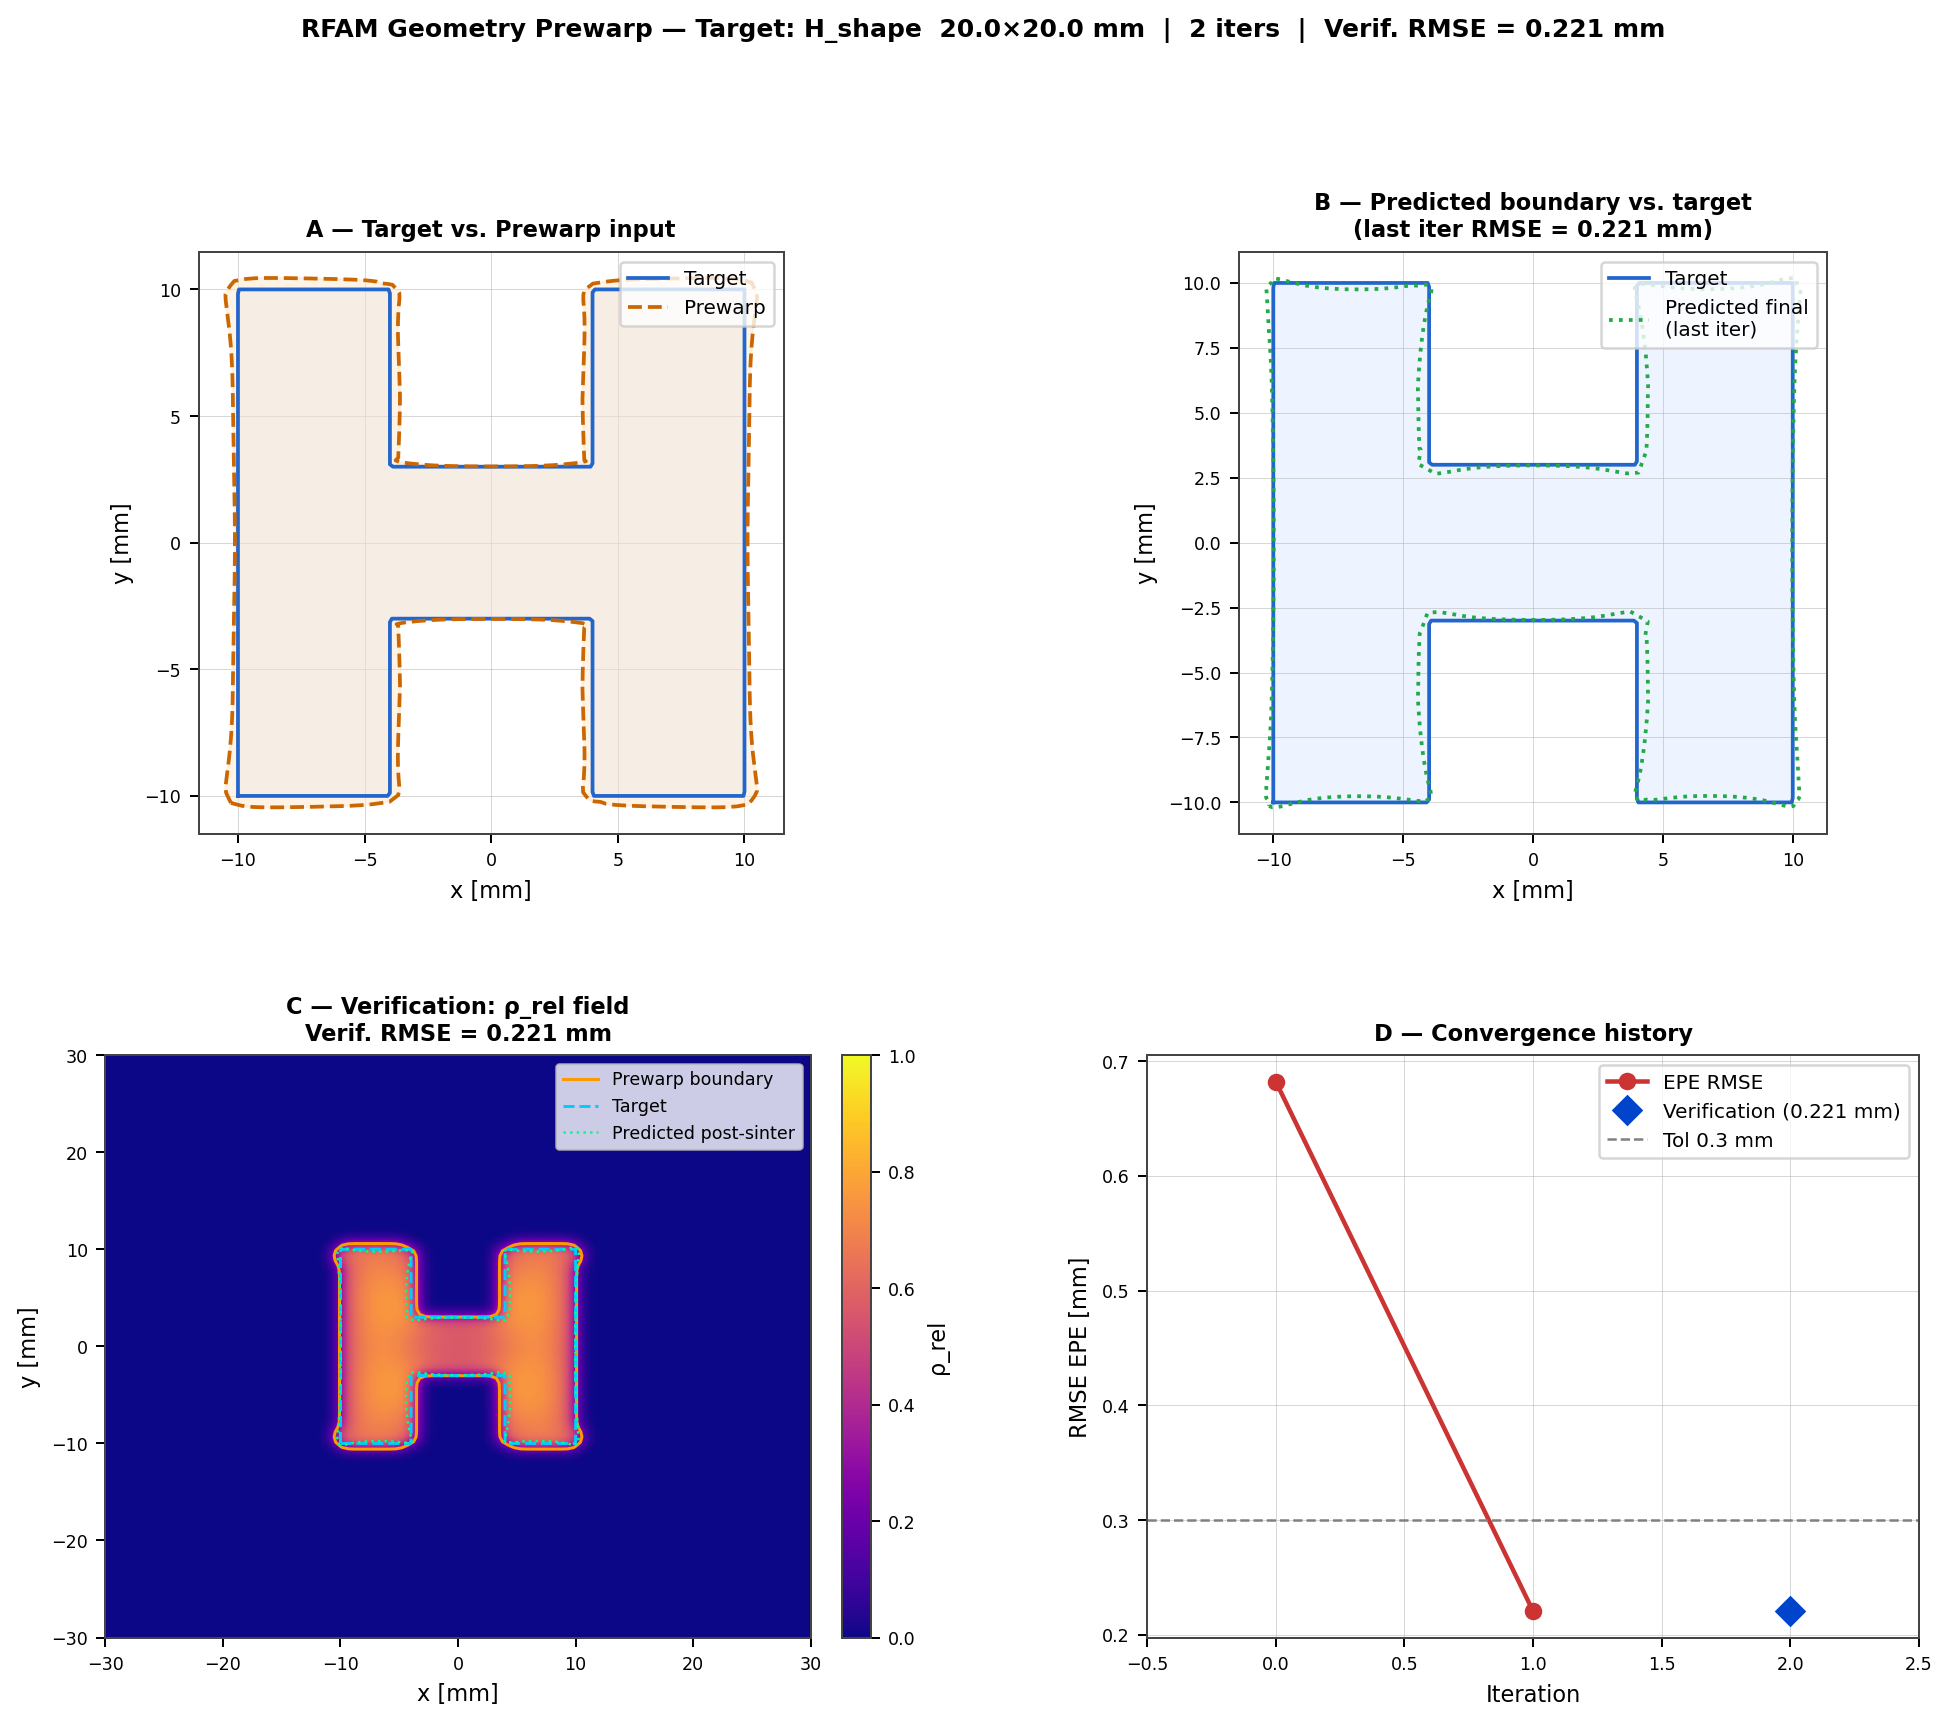
\includegraphics[width=0.8\linewidth]{fig_prewarp_H.png}
  \vspace{0.4em}
  \begin{itemize}
    \item RMSE: \SI{0.682}{\milli\meter} $\rightarrow$ \SI{0.221}{\milli\meter} (68\% reduction)
  \end{itemize}
\end{frame}

\begin{frame}{H-Shape: Baseline vs Combined}
  \centering
  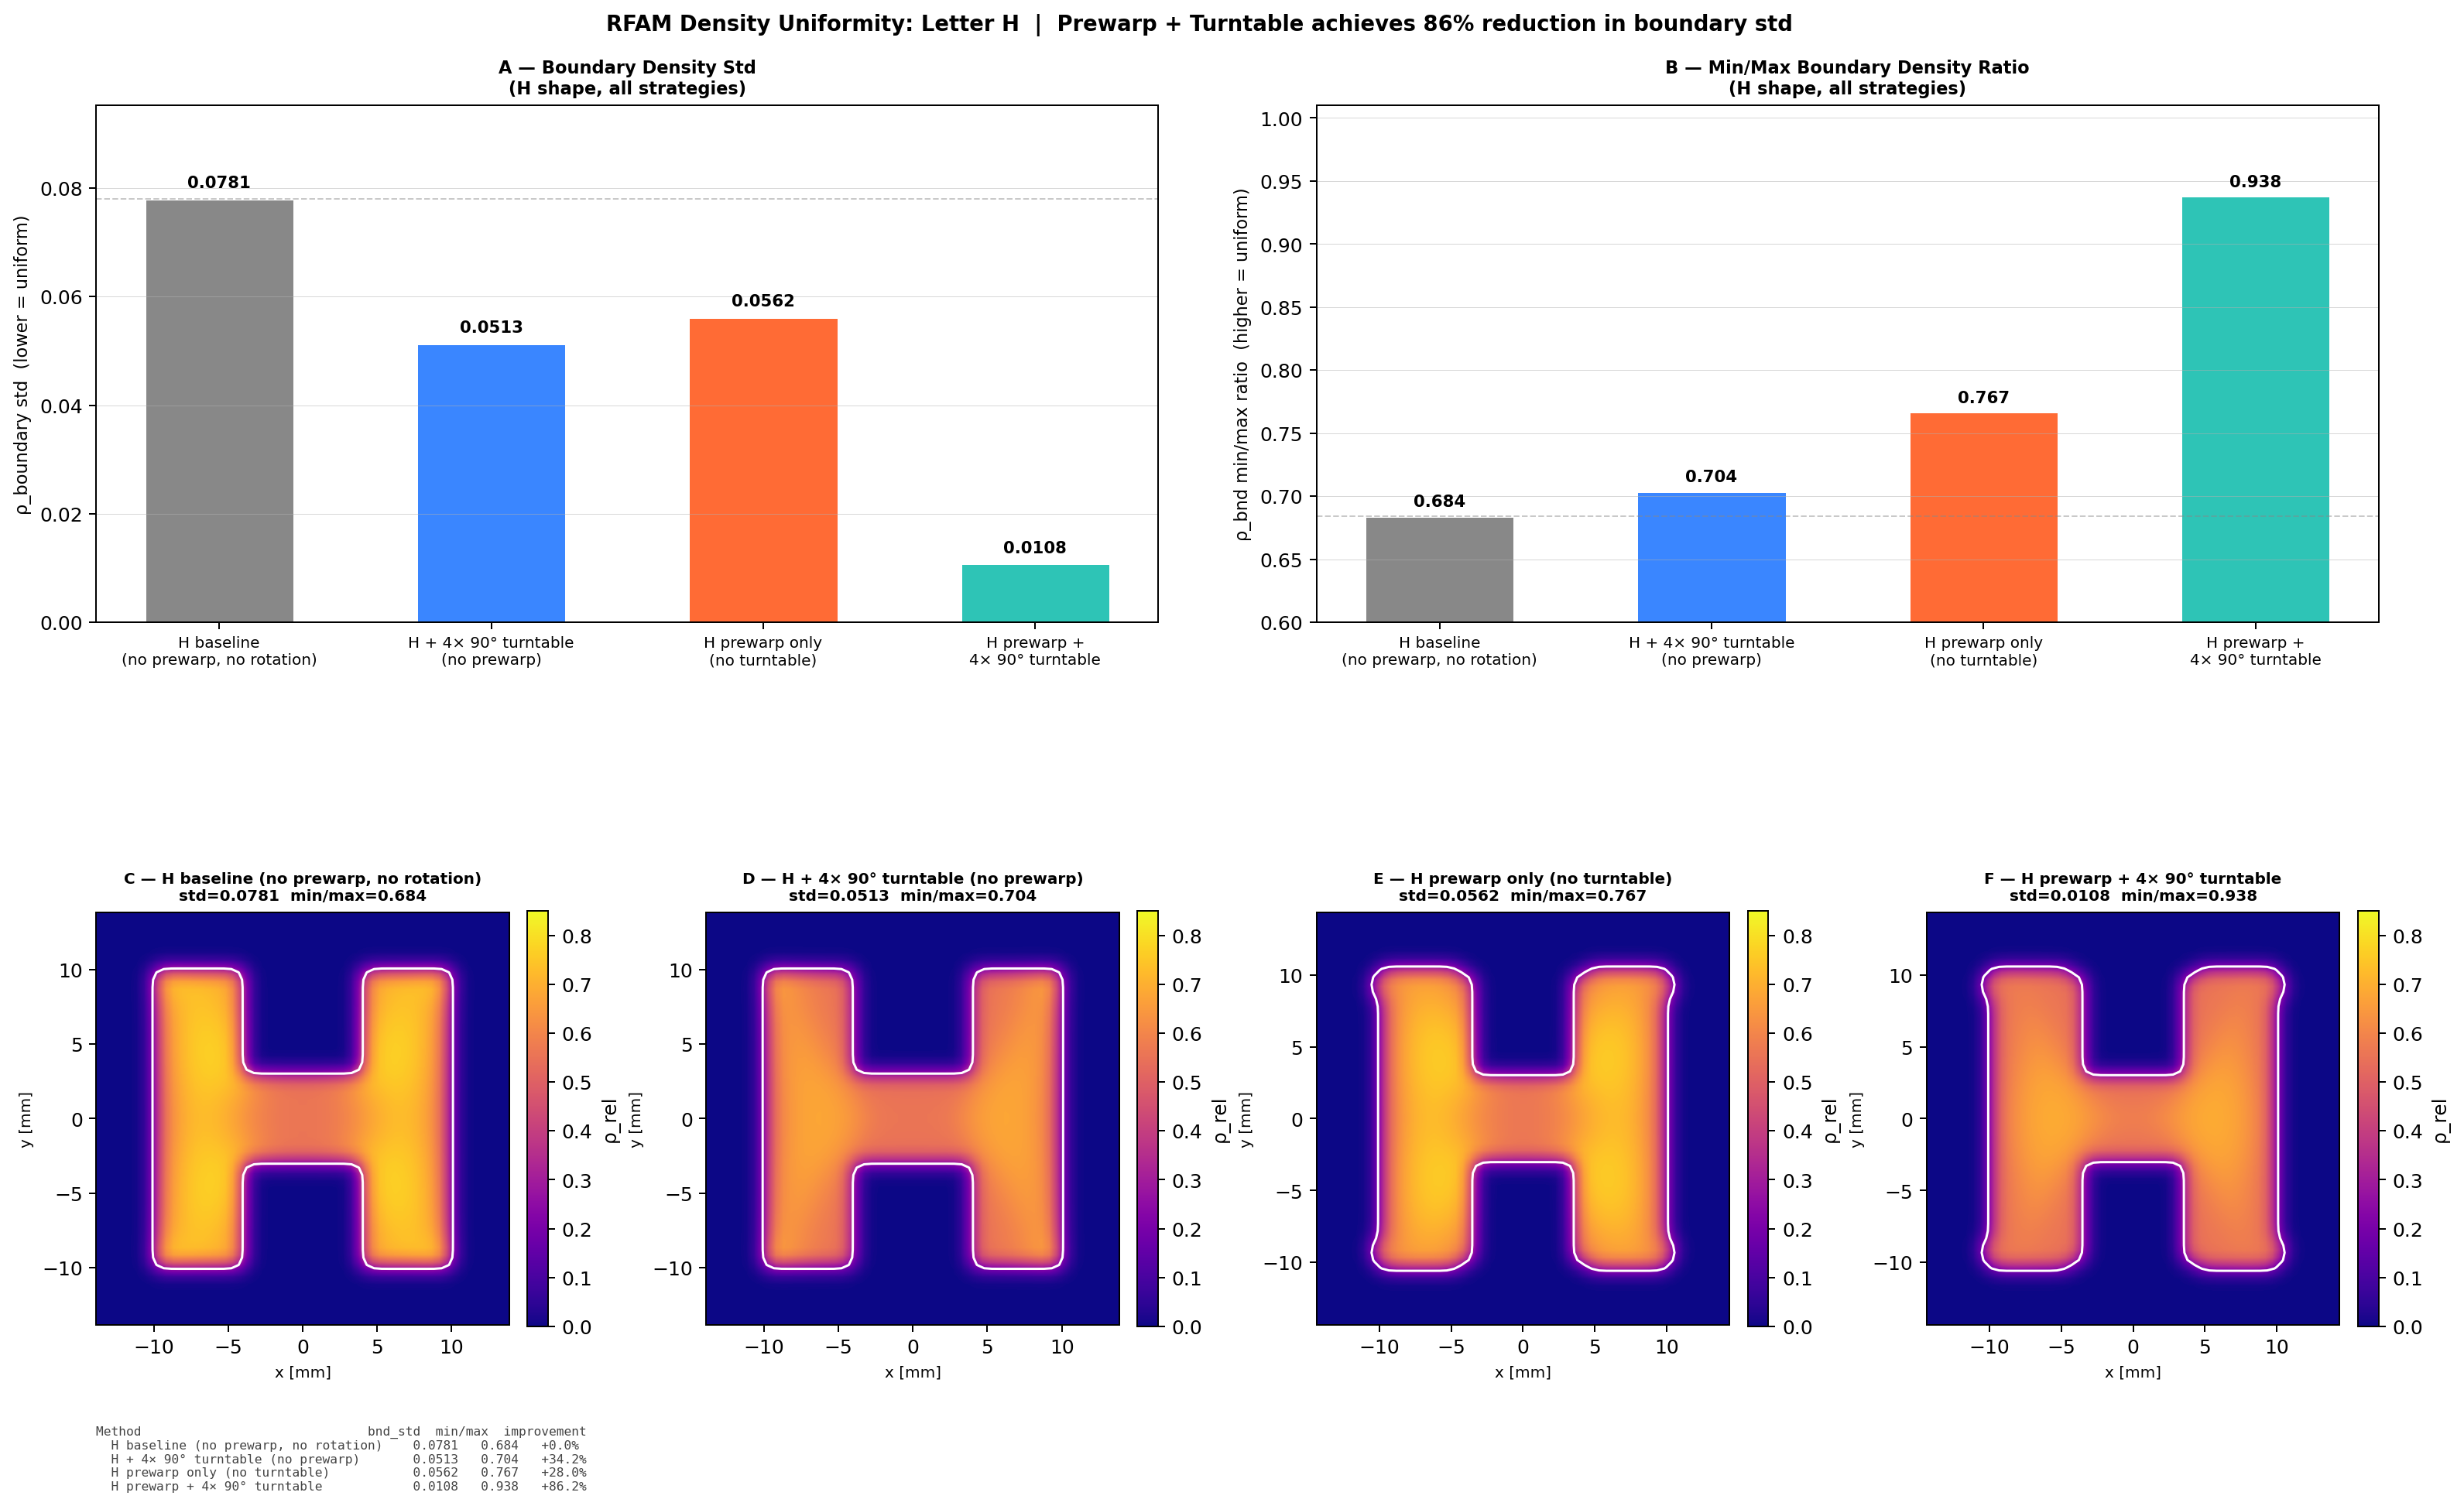
\includegraphics[width=\linewidth]{fig_H_uniformity.png}
\end{frame}

\begin{frame}{H-Shape Combined Five-Panel Summary}
  \centering
  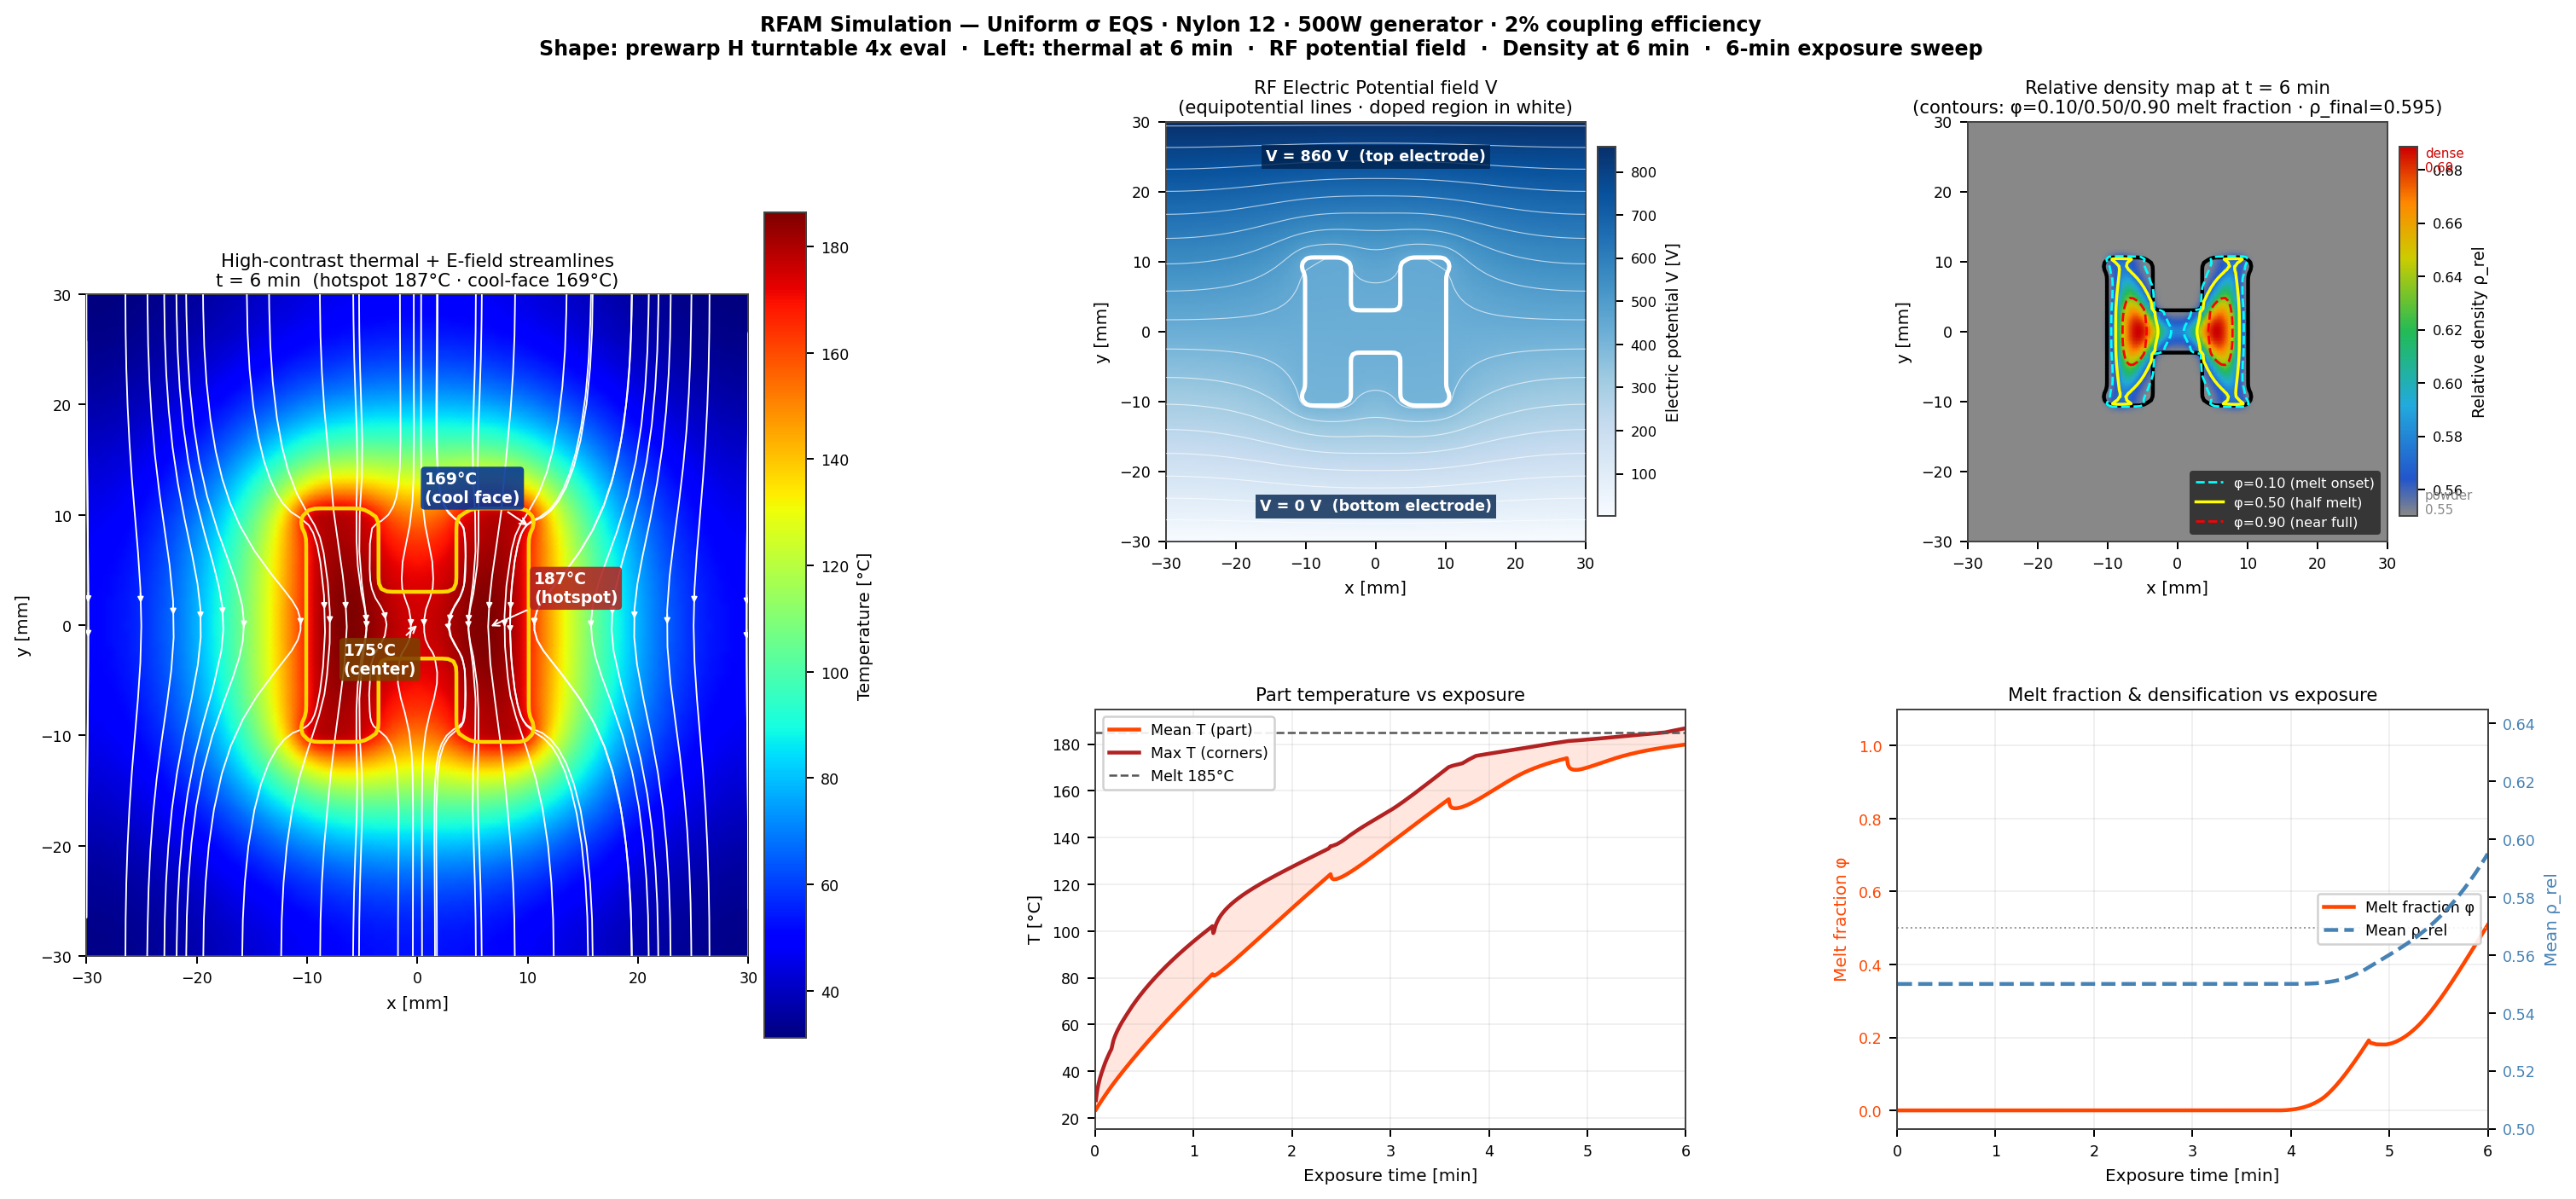
\includegraphics[width=\linewidth]{fig_H_combined_v5.png}
\end{frame}

\begin{frame}{Key Quantitative Outcomes}
  \begin{itemize}
    \item Square:
    \begin{itemize}
      \item baseline $\bndstd = 0.0724$
      \item prewarp + 4$\times$90$^\circ$: $\bndstd = 0.0253$ (65\% reduction)
    \end{itemize}
    \item H-shape:
    \begin{itemize}
      \item baseline $\bndstd = 0.0781,\ r_{\mathrm{bnd}}=0.684$
      \item prewarp + 4$\times$90$^\circ$: $\bndstd = 0.0108,\ r_{\mathrm{bnd}}=0.938$
      \item 86\% boundary non-uniformity reduction
    \end{itemize}
    \item Positive synergy: combined effect exceeds sum of individual prewarp + turntable effects.
  \end{itemize}
\end{frame}

\begin{frame}{Conclusions}
  \begin{itemize}
    \item RFAM non-uniformity is fundamentally geometric and orientation-dependent.
    \item EPE-based prewarp is effective for geometric correction and partial uniformity improvement.
    \item Spike assists are limited in practical RFAM use.
    \item Turntable averaging is effective, and strongest when paired with prewarp.
    \item Combined strategy delivers near-uniform boundary densification for challenging shapes.
  \end{itemize}
\end{frame}

\begin{frame}{Backup: Main Equations}
  \small
  \[
    \Qrf = \frac{1}{2}\sigma |\nabla V|^2,\qquad
    \bndstd = \mathrm{std}\left(\{\rhorel[i,j]:(i,j)\in\mathcal{B}\}\right),\qquad
    r_{\mathrm{bnd}}=\frac{\min_{\mathcal{B}}\rhorel}{\max_{\mathcal{B}}\rhorel}
  \]
  \[
    \hat{B}[i]=P_k[i]-s[i]\Leff \hat{n}_i,\qquad
    P_{k+1}[i]=P_k[i]+\alpha \EPE[i]\hat{n}_i
  \]
\end{frame}

\end{document}
